% Settings for the default beamer theme
\documentclass[english, aspectratio=169]{beamer}
\usepackage[T1]{fontenc}
\usepackage[utf8]{inputenc}
\usepackage{tabularx}
\usepackage{babel}
\usepackage[ruled,vlined]{algorithm2e}
\SetAlgorithmName{Algoritmus}{algoritmus}{List of Algorithms}
\setcounter{secnumdepth}{3}
\setcounter{tocdepth}{3}

\makeatletter

\newcommand\makebeamertitle{\frame{\maketitle}}

% (ERT) argument for the TOC
\AtBeginDocument{%
  \let\origtableofcontents=\tableofcontents
  \def\tableofcontents{\@ifnextchar[{\origtableofcontents}{\gobbletableofcontents}}
  \def\gobbletableofcontents#1{\origtableofcontents}
}

% Theme settings
\usetheme{Frankfurt}
\usecolortheme{default}
\usefonttheme[onlymath]{serif}

% Template settings
\setbeamertemplate{navigation symbols}{}
\setbeamertemplate{blocks}[rounded][shadow=false]
\setbeamertemplate{title page}[default][colsep=-4bp, rounded=true, shadow=false]
\makeatother

% Define a custom darker red color
\definecolor{DarkerRed}{RGB}{139,0,0} % Adjust the RGB values as needed

% Use the newly defined color in Beamer theme elements
\setbeamercolor{structure}{fg=DarkerRed} % Changes basic structural elements to Darker Red
\setbeamercolor{title in head/foot}{bg=DarkerRed} % Changes the title in header/footer to Darker Red


\begin{document}

% Title page
\section{Bevezetés}
\title[]{Üzleti Elemzések Módszertana}
\subtitle{5. Előadás: Együttes tanulás}
\author[Kuknyó Dániel]{Kuknyó Dániel\\Budapesti Gazdasági Egyetem}
\date{2023/24\\2.félév}
\makebeamertitle

% Table of contents slide
\begin{frame}
\tableofcontents{}
\end{frame}

% Table of contents of the current section
\begin{frame}
\tableofcontents[currentsection]
\end{frame}

\begin{frame}{Az együttes tanulás mögötti intuíció}
\begin{columns}
\begin{column}{.5\textwidth}
\begin{itemize}
	\item Egy gazda szeretné lemérni, milyen a hőmérséklet a szőlős birtokán. 
	\item A birtok egy hegyoldalban fekszik, ezért a szőlőtőkéket eltérő időjárási hatások érik.
\end{itemize}
\end{column}
\begin{column}{.5\textwidth}
\begin{center}
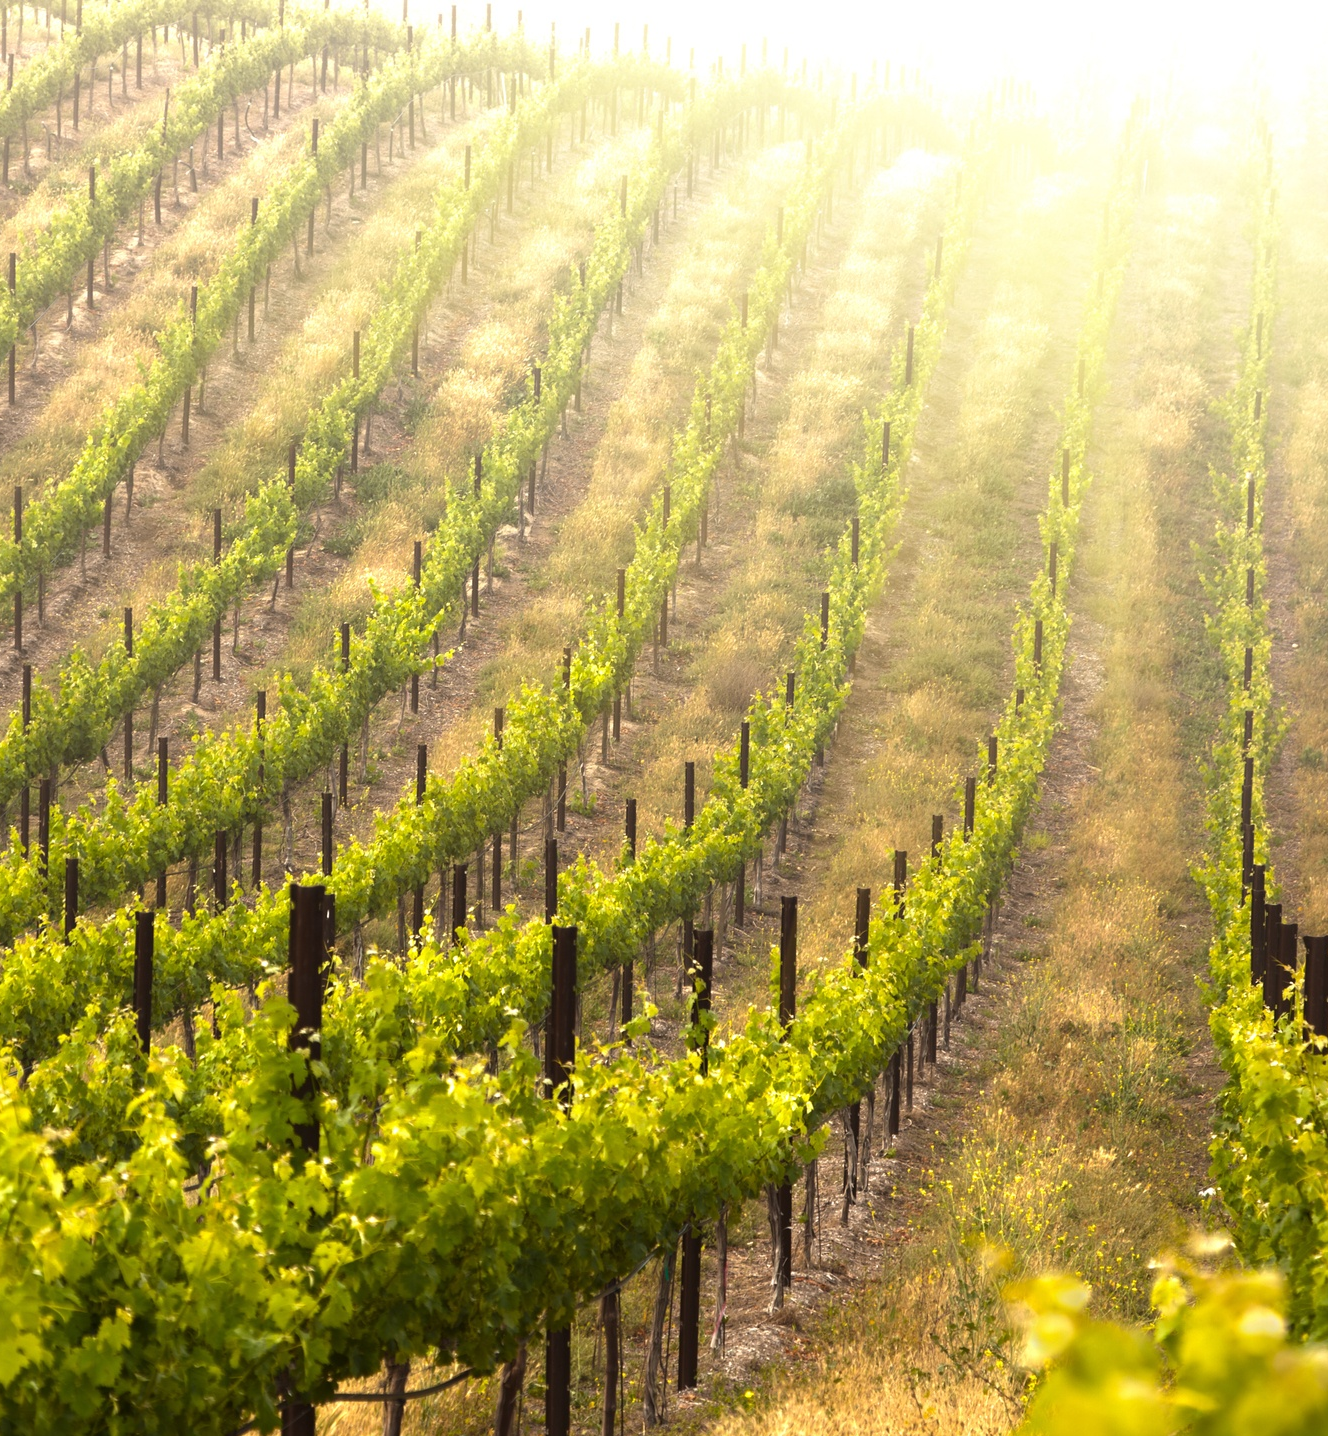
\includegraphics[width=7cm, height=5cm, keepaspectratio]{images/ensemble_2.png}
\end{center}
\end{column}
\end{columns}
\end{frame}

\begin{frame}{Példa: szavazó osztályozók}
\begin{columns}
\begin{column}{.5\textwidth}
A következő példában 10 osztályozó modell feladata, hogy megbecsüljék, melyik oldalára fog esni egy torzított pénzérme.\par\medskip
A pénzérme 51\% valószínűséggel esik fejre, 49\% eséllyel pedig írásra.\par\medskip
1000 dobás után 75\%, hogy a modellek valószínűsége fejt fog szavazni. Ugyanez a valószínűség 10000 dobás után 97\%.\par\medskip
A szavazó osztályozók nagyobb pontosságot érnek el együttesen, mint a modellcsoport bármelyik tagja. 
\end{column}
\begin{column}{.5\textwidth}
\begin{center}
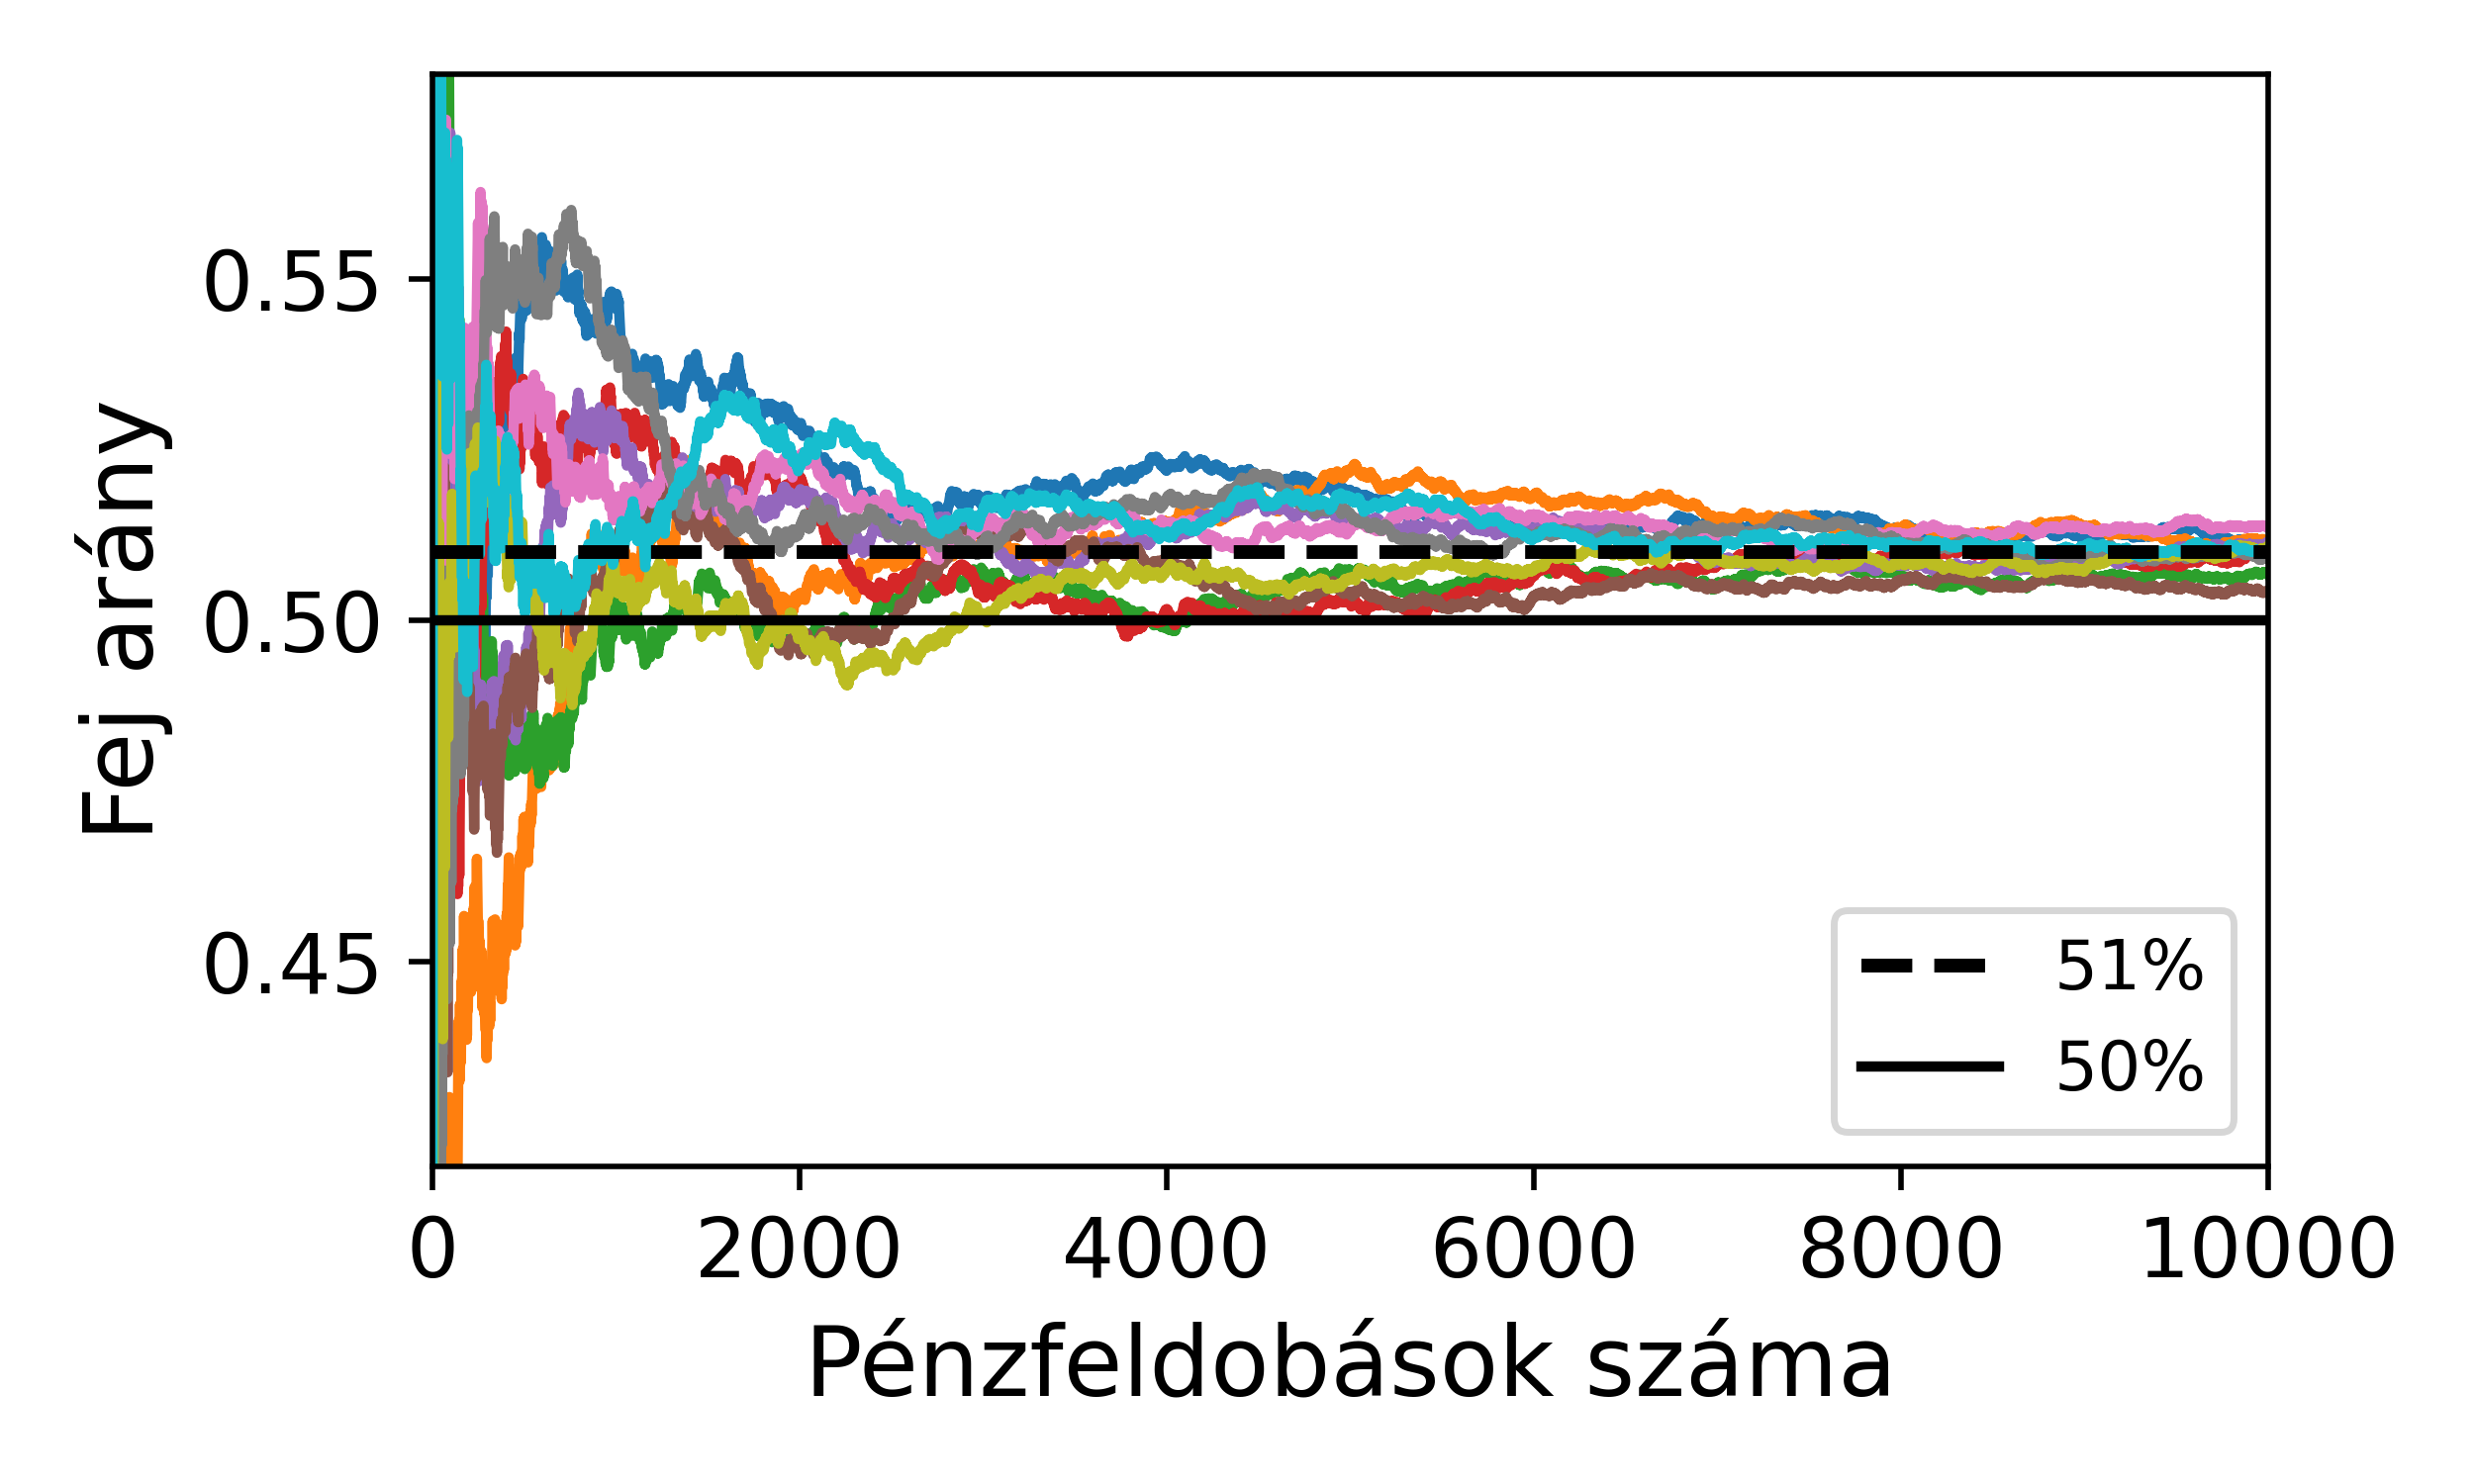
\includegraphics[width=7cm, height=7cm, keepaspectratio]{images/ensemble_1.png}
\end{center}
\end{column}
\end{columns}
\end{frame}

\begin{frame}{Szavazó osztályozók}
\begin{columns}
\begin{column}{.5\textwidth}
A szavazó osztályozó kifejezés modellek egy csoportjára utal, amelyben a modellek \textbf{egymástól függetlenül képesek predikciót adni} egy adott mintaegyedre vonatkozóan.\par\smallskip
A szavazó osztályozó a végső predikciót úgy állítja elő, hogy \textbf{a benne lévő modellek predikcióit aggregálja} valamilyen módszertan szerint (pl. átlagolás, módusz, medián) kiválasztja belőle a leggyakoribb elemet. 
\end{column}
\begin{column}{.5\textwidth}
\begin{center}
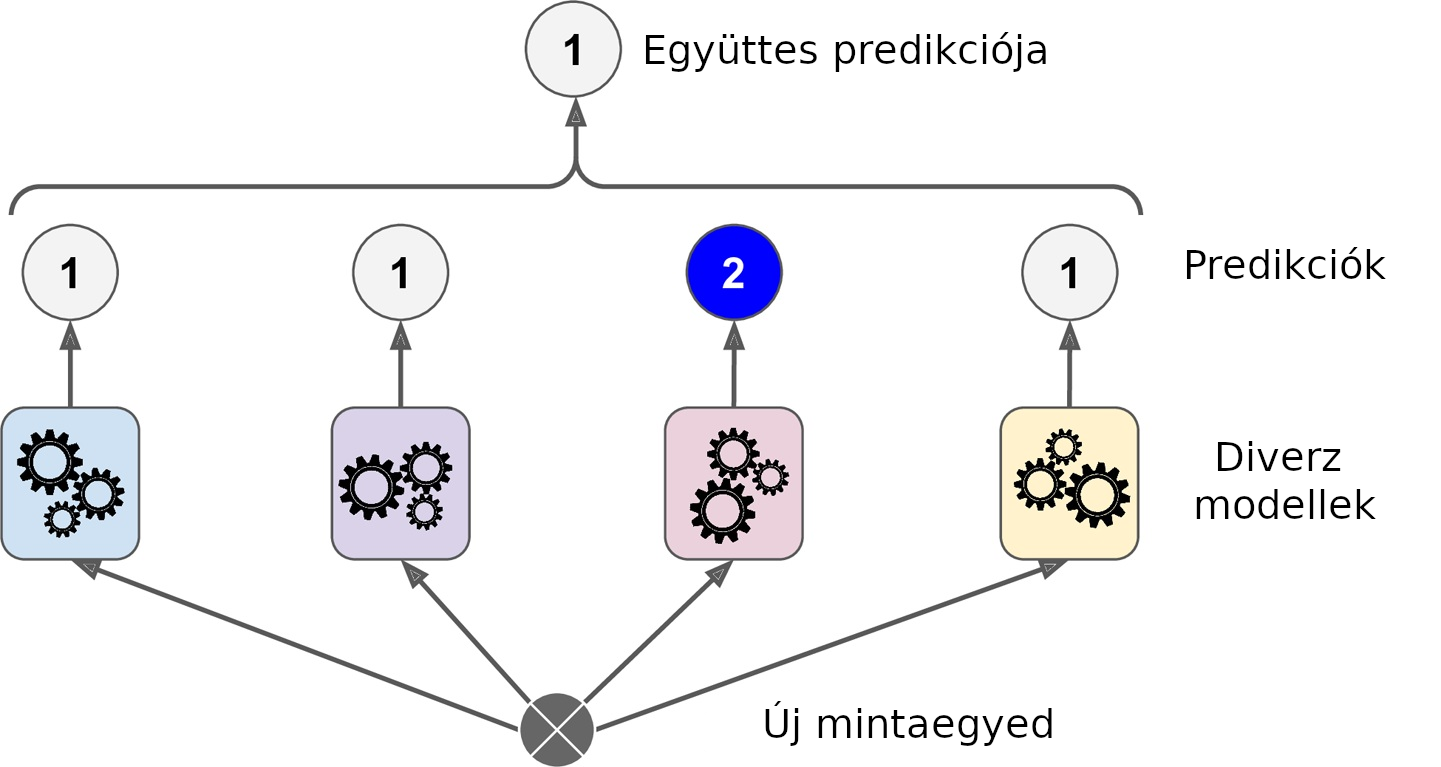
\includegraphics[width=7cm, height=7cm, keepaspectratio]{images/ensemble_3.png}
\end{center}
\end{column}
\end{columns}
\end{frame}

\begin{frame}{Bagging és Pasting}
\begin{columns}
\begin{column}{.5\textwidth}
Az együttes tanuló modellek taníthatók az adathalmaz különböző részhalmazain. Ez robusztusabb modellt fog eredményezni, ami jobb általánosító képességeket jelent éles felhasználásban.
\only<1>{\begin{block}{Bagging}
Együttes tanulási módszer, melyben a modellek \textbf{visszatevés nélküli mintavétellel} kapják meg a saját tanító mintájukat.
\end{block}} 
\only<2>{\begin{block}{Pasting}
Együttes tanulási módszer, melyben a modellek \textbf{visszatevéses mintavétellel} kapják meg a saját tanító mintájukat.
\end{block}}
\end{column}
\begin{column}{.5\textwidth}
\begin{center}
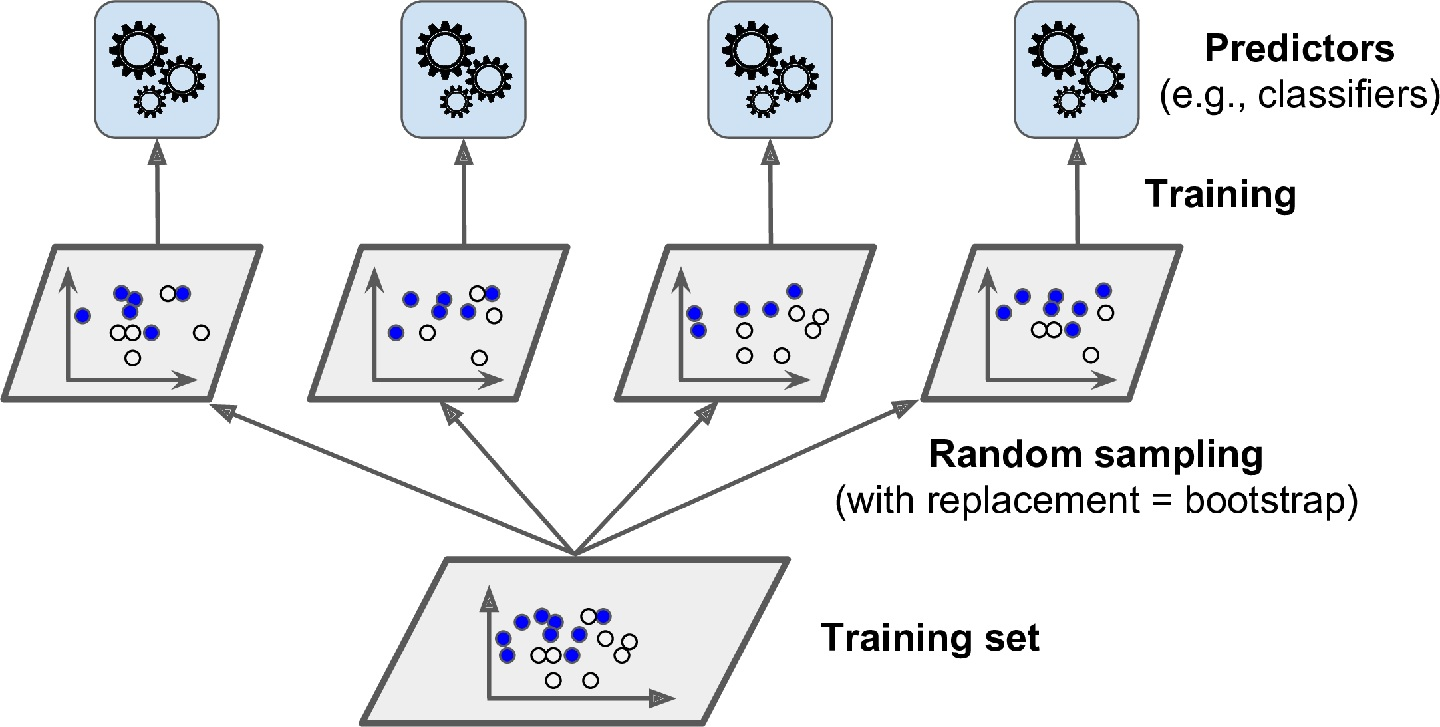
\includegraphics[width=7cm, height=7cm, keepaspectratio]{images/ensemble_4.png}
\end{center}
\end{column}
\end{columns}
\end{frame}

\begin{frame}{Bagging hatása a döntési határokra}
A bal oldali ábrán egyetlen döntési fa határai láthatóak, a jobb oldalin pedig több bagging technikával tanított döntési fának a határait. A bagging modellcsoport egyértelműen jobb általánosító képességekkel rendelkezik mint a döntési fa.
\begin{center}
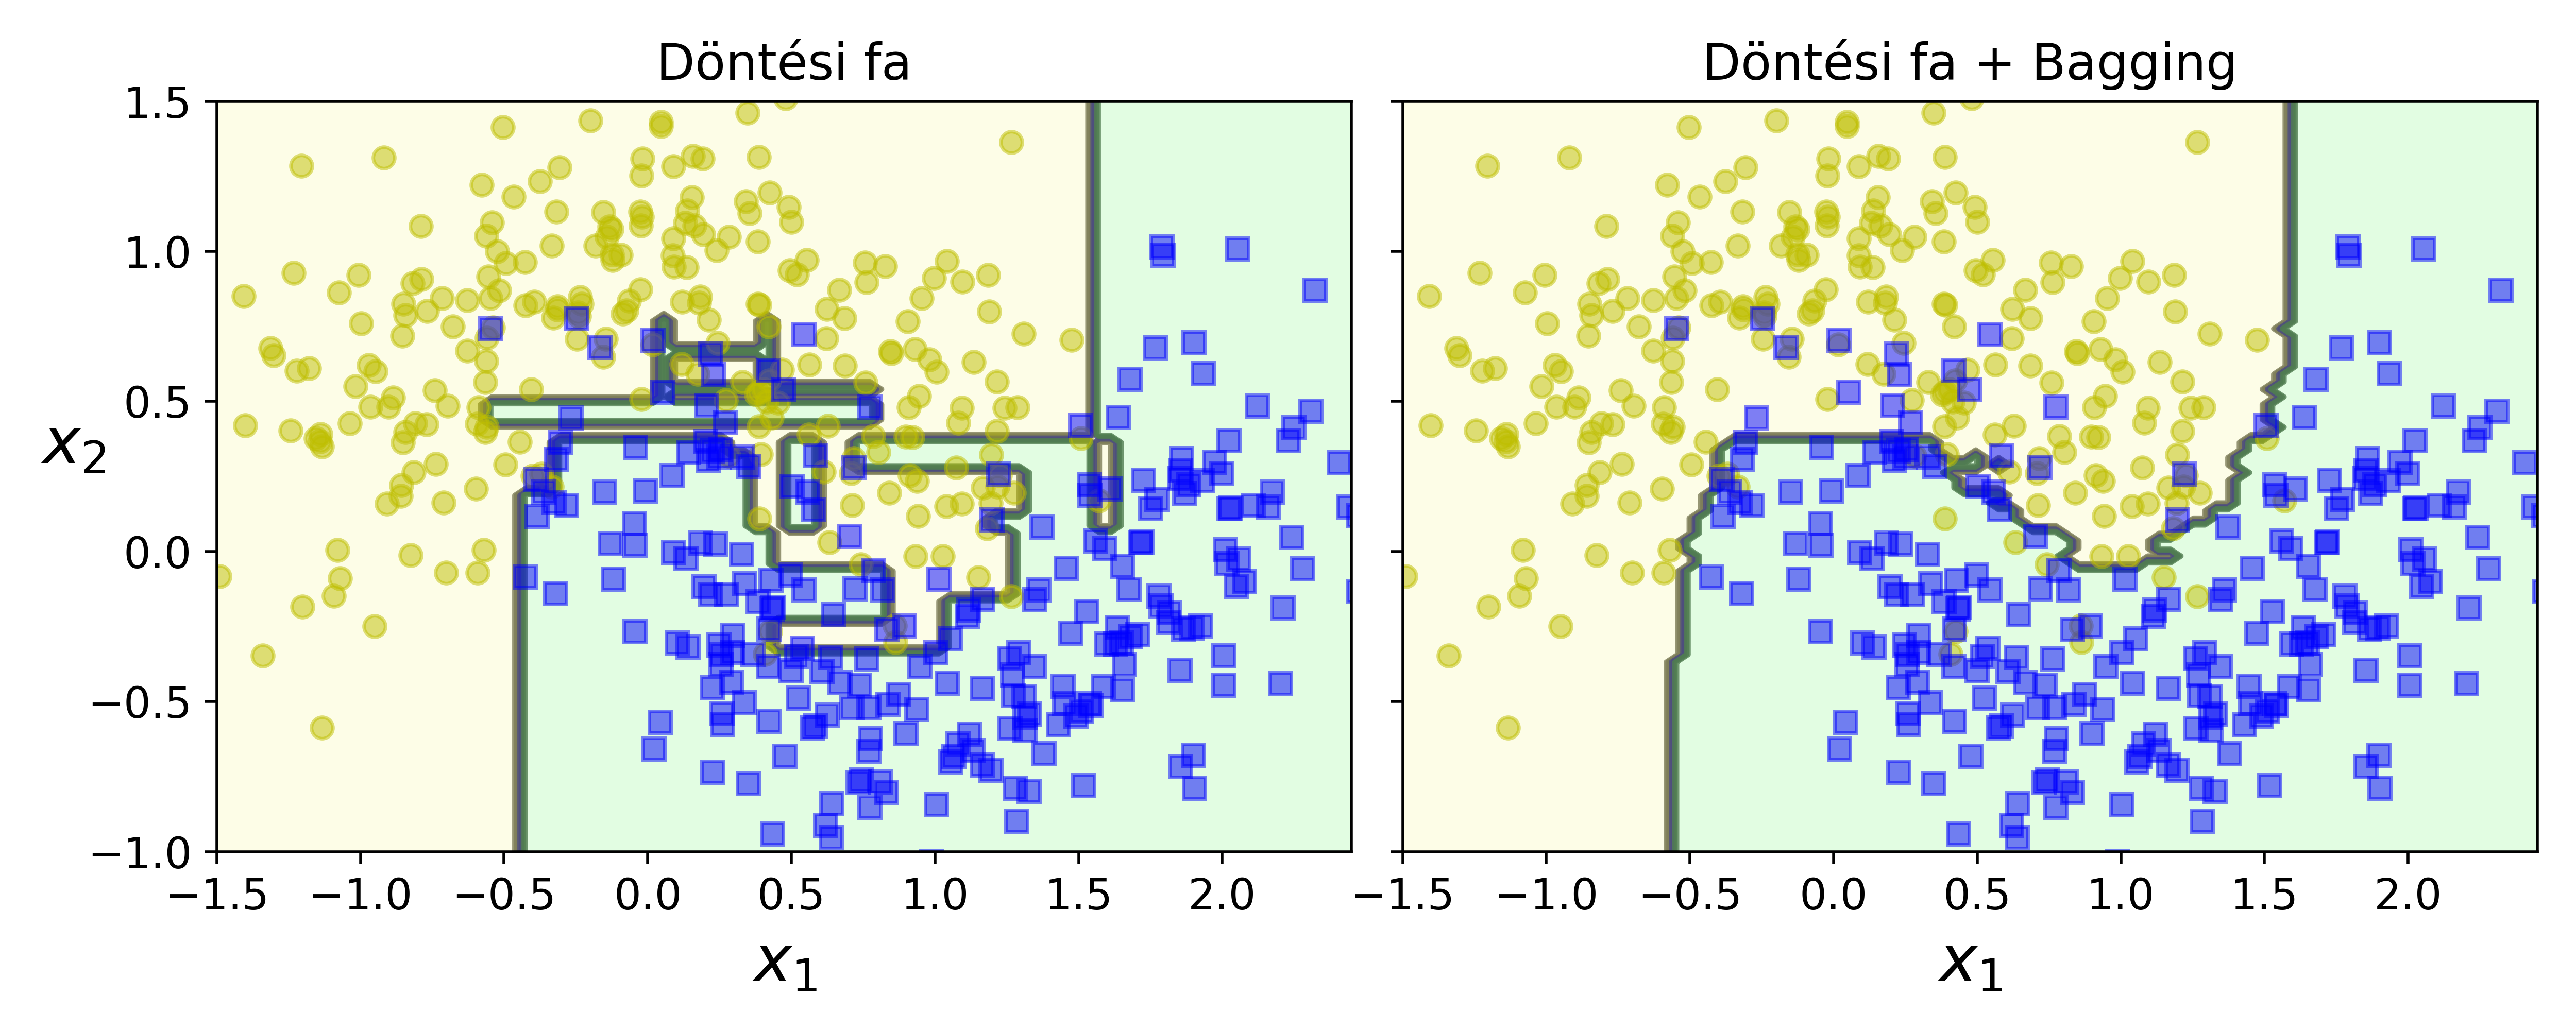
\includegraphics[width=12cm, height=7cm, keepaspectratio]{images/ensemble_5.png}
\end{center}
\end{frame}

\section{Adaptív turbózás}

\begin{frame}
\tableofcontents[currentsection]
\end{frame}

\begin{frame}{Adaptív turbózás}
\begin{columns}
\begin{column}{.5\textwidth}
\begin{block}{Adaptív turbózás}
Az együttes tanulás súlyozott változata. A modellek szekvenciálisan állnak elő olyan módon, hogy az új modell mindig tanul az elődje hibájából. 
\end{block}
\end{column}
\begin{column}{.5\textwidth}
\begin{algorithm}[H]
\caption{Adaptív turbózás}
\SetAlgoLined
\begin{enumerate}
	\item Kezdeti súlyok rekordokhoz rendelése
	\item Modell illesztés minden változóra
	\item Legjobb modell kiválasztása
	\item Modell súlyozása
	\item Egyedsúlyok frissítése
	\item Adathalmaz újramintázása
	\item Iteráció kilépésig
\end{enumerate}
\end{algorithm}
\end{column}
\end{columns}
\end{frame}

\begin{frame}{Adaptív turbózás: lépésről lépésre}
\begin{columns}
\begin{column}{.5\textwidth}
Az Adaptív turbózás algoritmusa:
\begin{enumerate}
	\item Az algoritmus minden mintaegyedhez $w=\frac{1}{n}$ kezdeti súlyt rendel, ahol $n$ a minta halmaz mérete.
	\item Minden $x$ változóra egy döntési tönk kerül illesztésre. Ez egy lineáris döntési határ minden változóra. 
	\item Az a döntési tönk kerül kiválasztásra, amely a legjobban képes szeparálni az egyedeket. Ez ebben az esetben az $x_2$ változóhoz tartozó modell. 
\end{enumerate}
\end{column}
\begin{column}{.5\textwidth}
\begin{center}
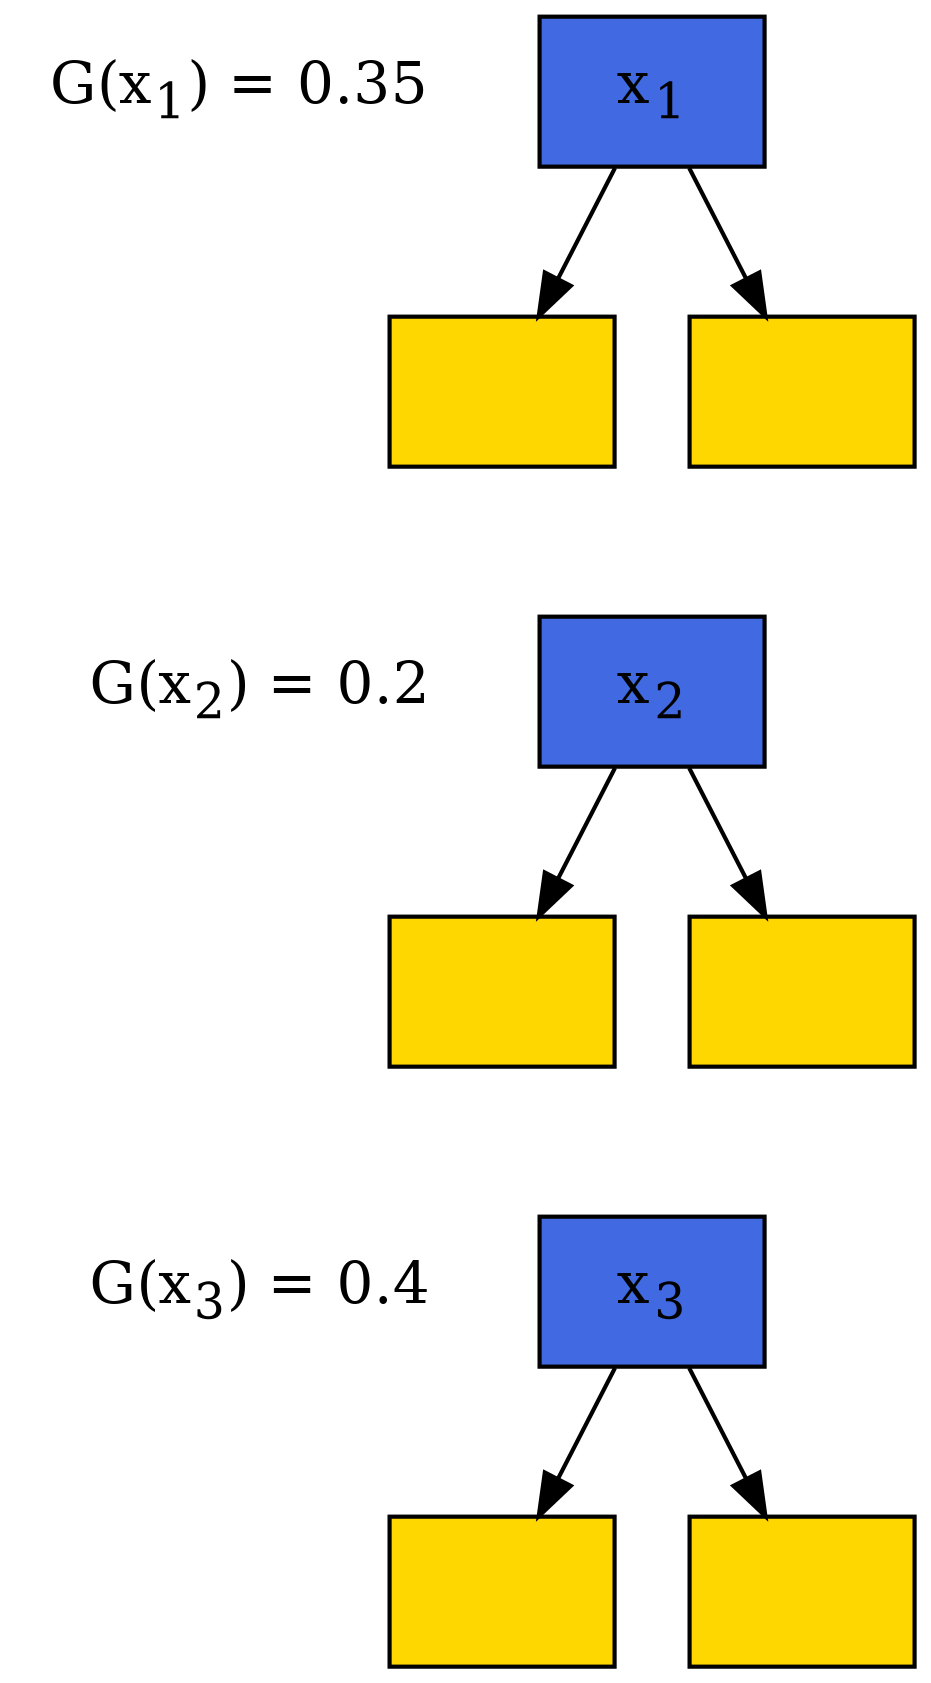
\includegraphics[width=7cm, height=7cm, keepaspectratio]{graphs/ensemble_1.png}
\end{center}
\end{column}
\end{columns}
\end{frame}

\begin{frame}{Adaptív turbózás: lépésről lépésre}
\begin{columns}
\begin{column}{.5\textwidth}
\begin{enumerate}
	\setcounter{enumi}{3}
	\item A modell súlyozása a teljes modellcsoportban. Egy tönk hibája azon mintaegyedek súlyainak összege, amelyeket helytelenül osztályozott:
	\begin{block}{Prediktor teljes hibája}
	\[
	r_j = \frac{\sum_{\underset{\hat{y}_j \neq y_i}{i=1}}^m w_i}{\sum_{i=1}^m w_i}
	\]
	\end{block}
	\begin{block}{Tönk súlya a modellben}
	\[
	W_j = \alpha \cdot log \left( \frac{1-r_j}{r_j} \right)
	\]
	Ahol $\alpha$ a tanulási sebesség.
	\end{block}
\end{enumerate}
\end{column}
\begin{column}{.5\textwidth}
\begin{center}
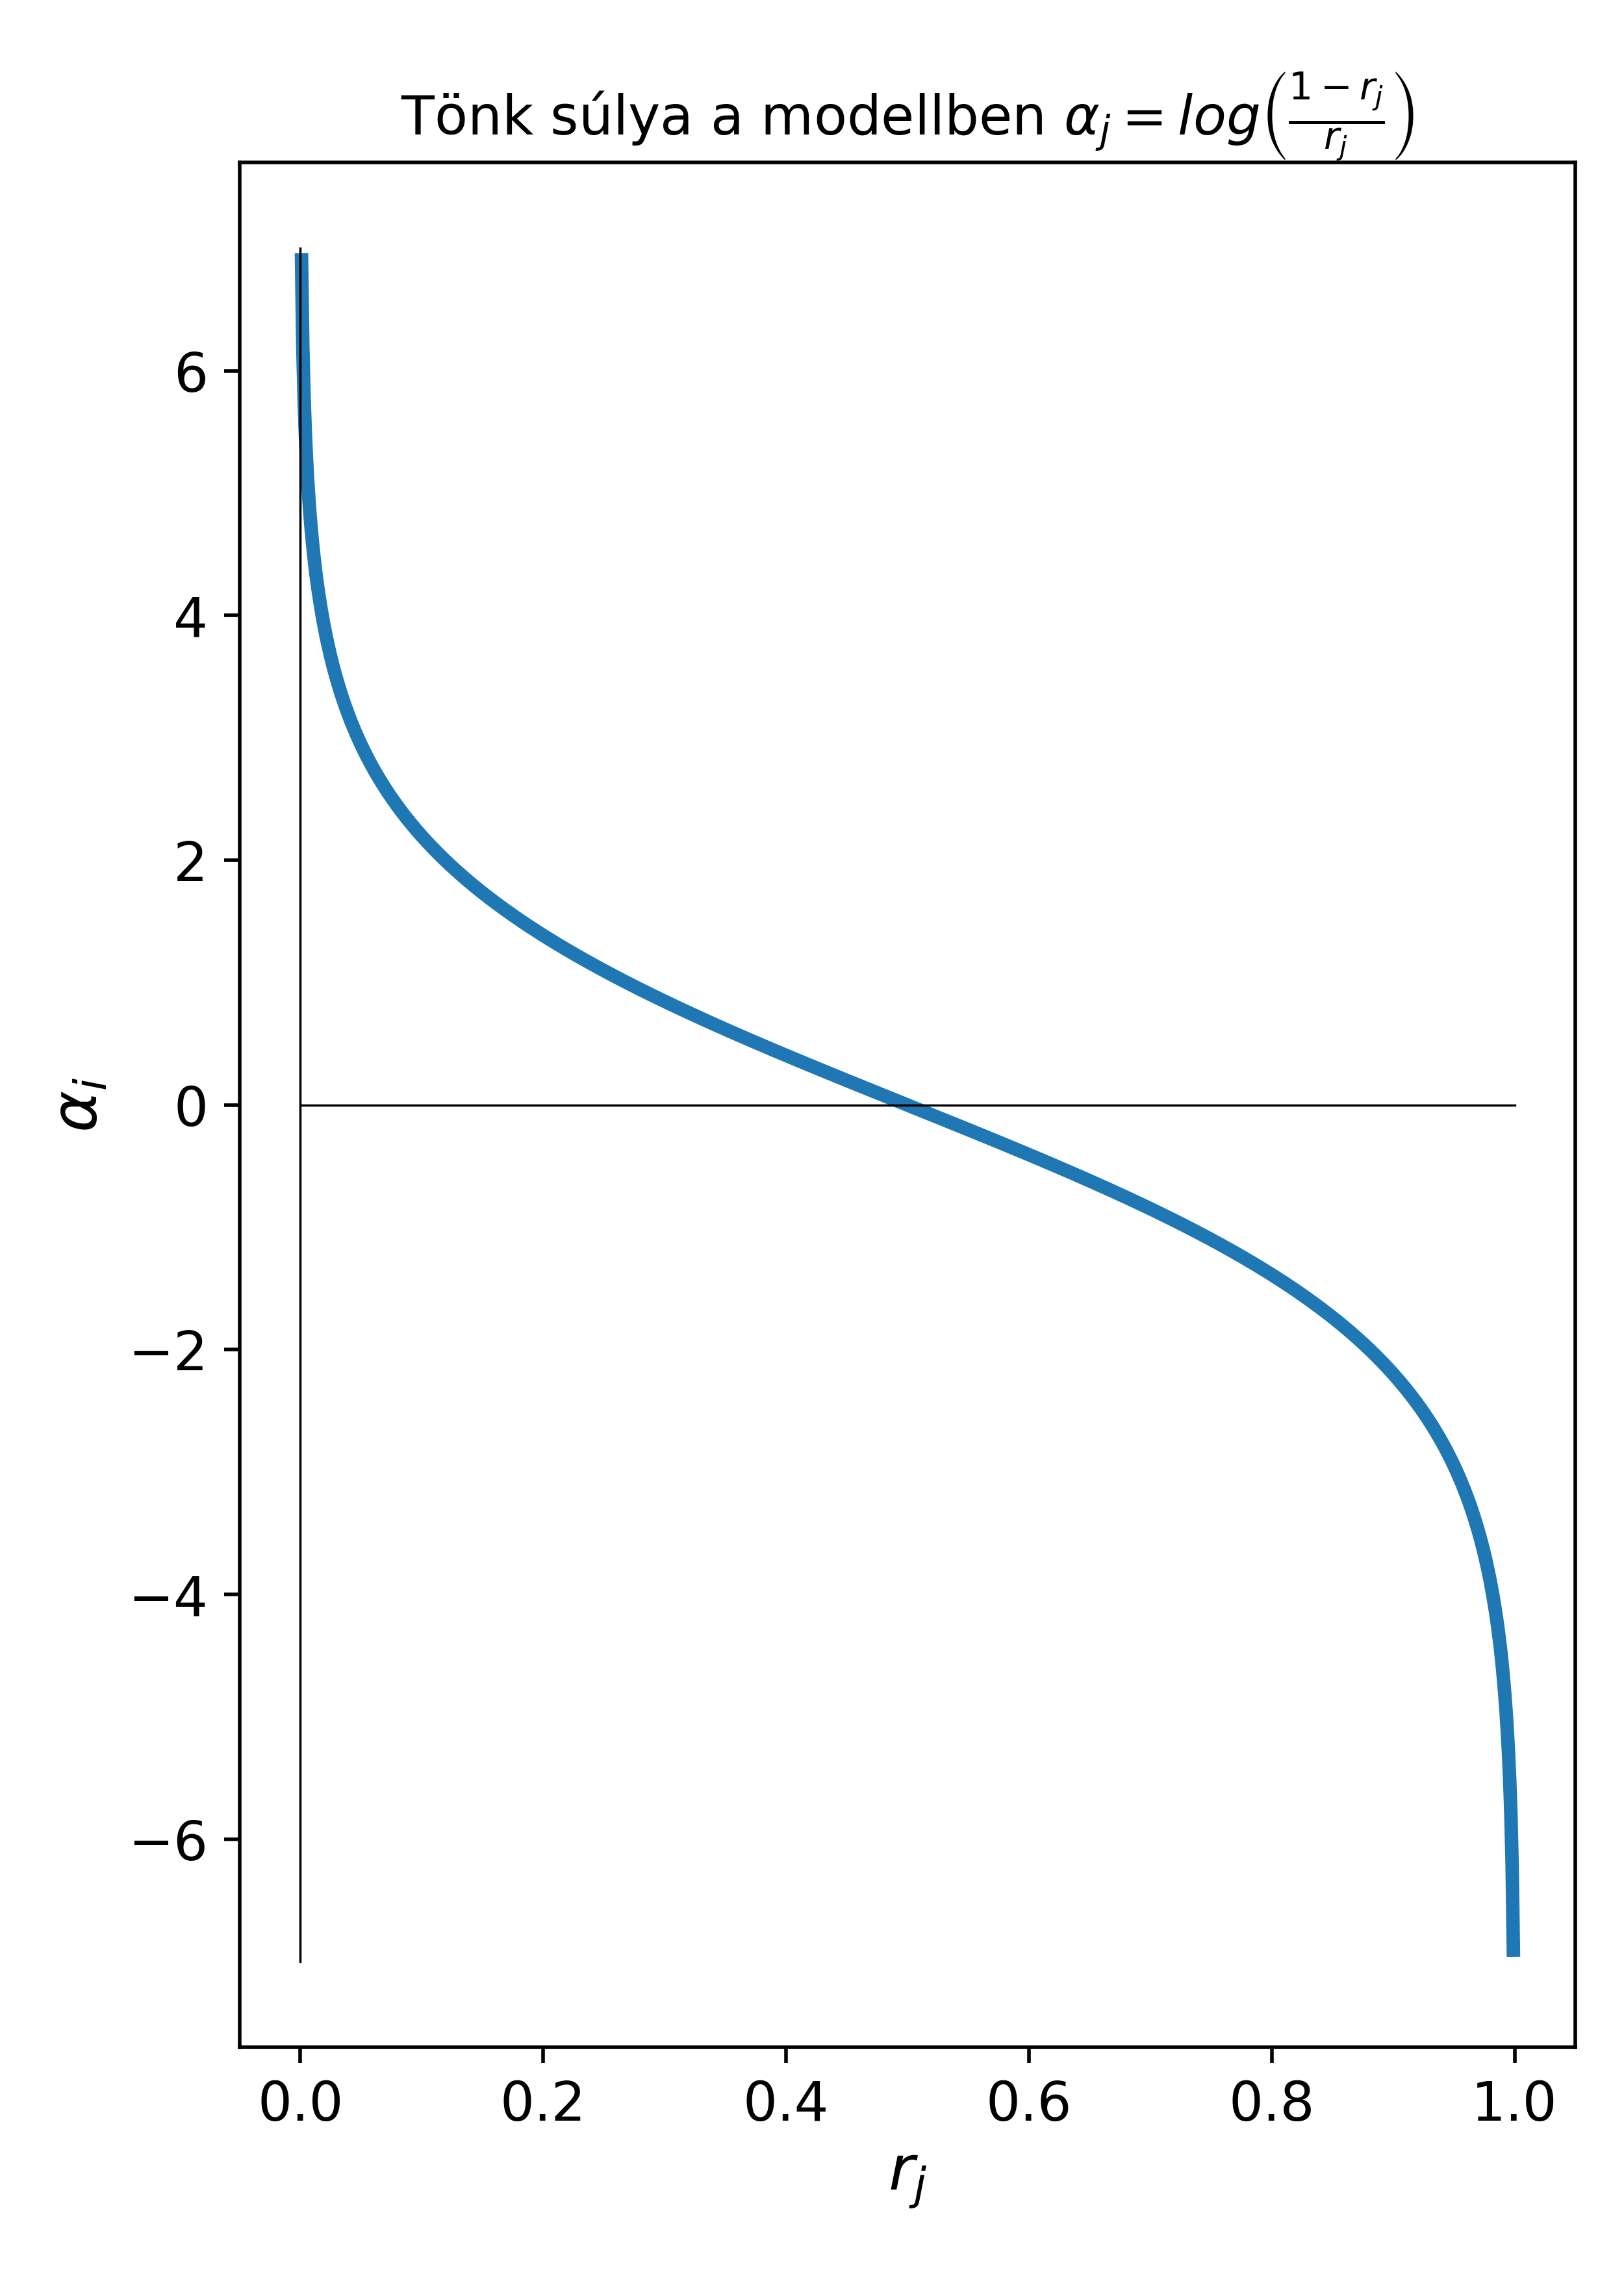
\includegraphics[width=7cm, height=7cm, keepaspectratio]{images/ensemble_6.png}
\end{center}
\end{column}
\end{columns}
\end{frame}

\begin{frame}{Adaptív turbózás: lépésről lépésre}
\begin{columns}
\begin{column}{.6\textwidth}
\begin{enumerate}
	\setcounter{enumi}{4}
	\item Az eljárás frissíti a mintaegyed súlyait.\par\smallskip 
	Minden helyesen beosztályozott mintaegyedre:
	\begin{block}{}
	\vspace{-0.2cm}
	\[
	w \leftarrow w \cdot e^{W_j}
	\]
	\end{block}
	Minden helytelenül beosztályozott mintaegyedre:
	\begin{block}{}
	\vspace{-0.2cm}
	\[
	w \leftarrow w \cdot e^{-W_j}
	\]
	\end{block}
	\item A létrejött egyedsúlyoknak megfelelő valószínűség eloszlást felhasználva az adathalmaz újramintázódik és eszerint kapja meg a következő fa a saját mintáját. 
	\item Az algoritmus a folyamatot addig ismétli, amíg el nem éri a kilépési kritériumot.
\end{enumerate}
\end{column}
\begin{column}{.4\textwidth}
\begin{center}
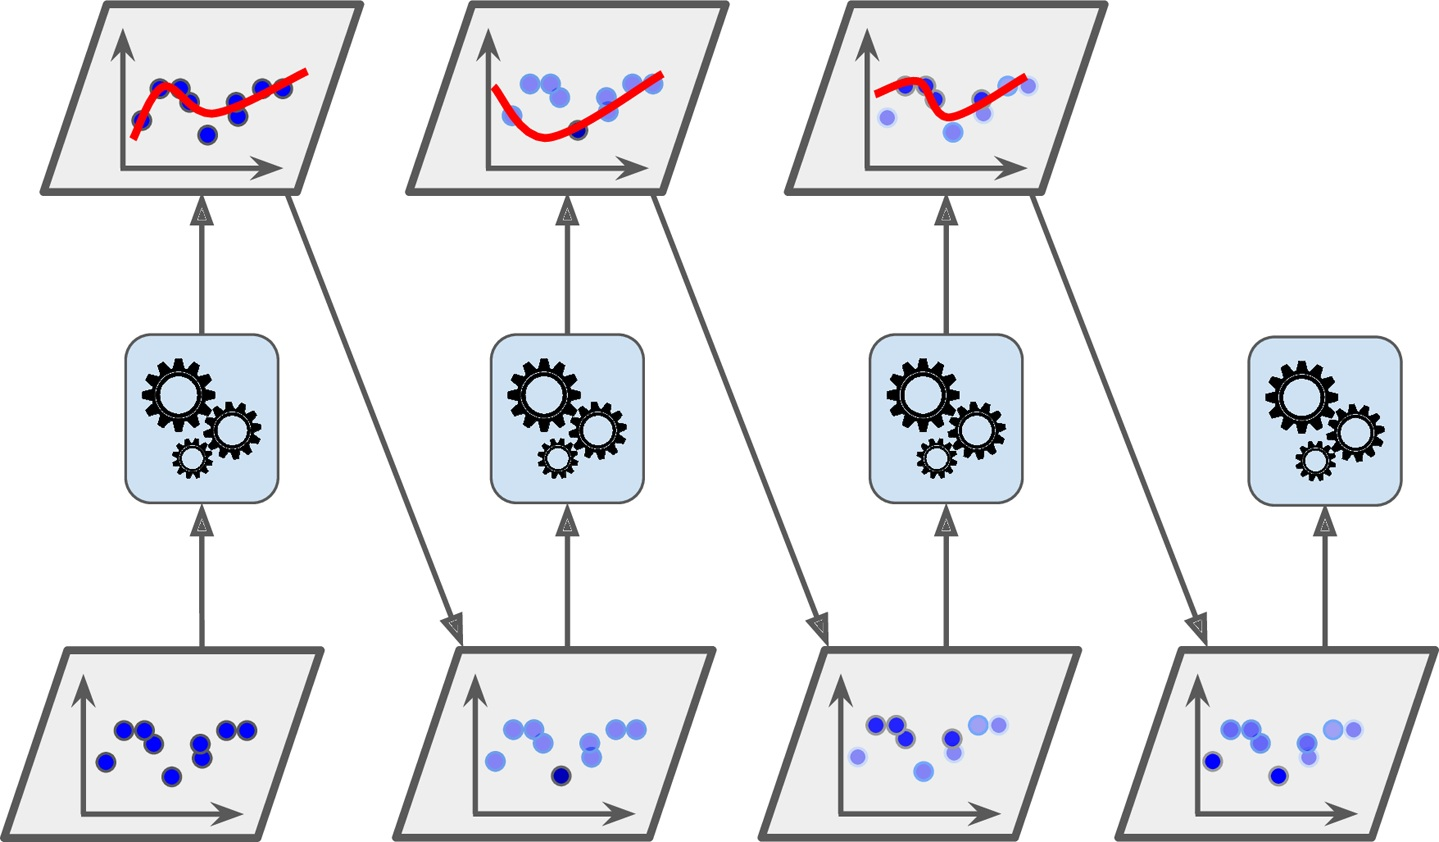
\includegraphics[width=6cm, height=7cm, keepaspectratio]{images/ensemble_7.png}
\end{center}
\end{column}
\end{columns}
\end{frame}

\begin{frame}{Az osztályozás eljárása}
\begin{columns}
\begin{column}{.5\textwidth}
Osztályozáskor minden létrejött döntési tönk létrehozza a saját predikcióját, és a különböző prediktorok szavazása által dől el, mi legyen a végső predikció.\par\medskip
Az egyed abba az osztályba lesz besorolva, amelyikhez tartozó tönkök súlyának összege a legnagyobb. 
\begin{block}{}
\[
\hat{y} = \underset{k}{argmax} \sum_{\underset{\hat{y}_j\left(x\right)=k}{j=1}}^N \alpha_j
\]
\end{block}
\only<1>{\vspace{0.55cm}}
\only<2>{A példában: $\hat{y}=B$}
\end{column}
\begin{column}{.5\textwidth}
\begin{center}
\includegraphics<1>[height=7cm, keepaspectratio]{graphs/ensemble_2.png}
\includegraphics<2>[height=7cm, keepaspectratio]{graphs/ensemble_3.png}
\end{center}
\end{column}
\end{columns}
\end{frame}

\begin{frame}{Adaptív turbózás a Moons halmazon}
\begin{columns}
\begin{column}{.5\textwidth}
A \texttt{make-moons} könyvtár egy nemlineárisan szeparálható adathalmazt generál.\par\medskip
A következő ábrán egy döntési fa alapú adaptív turbózó döntési határai láthatók.
\end{column}
\begin{column}{.5\textwidth}
\begin{center}
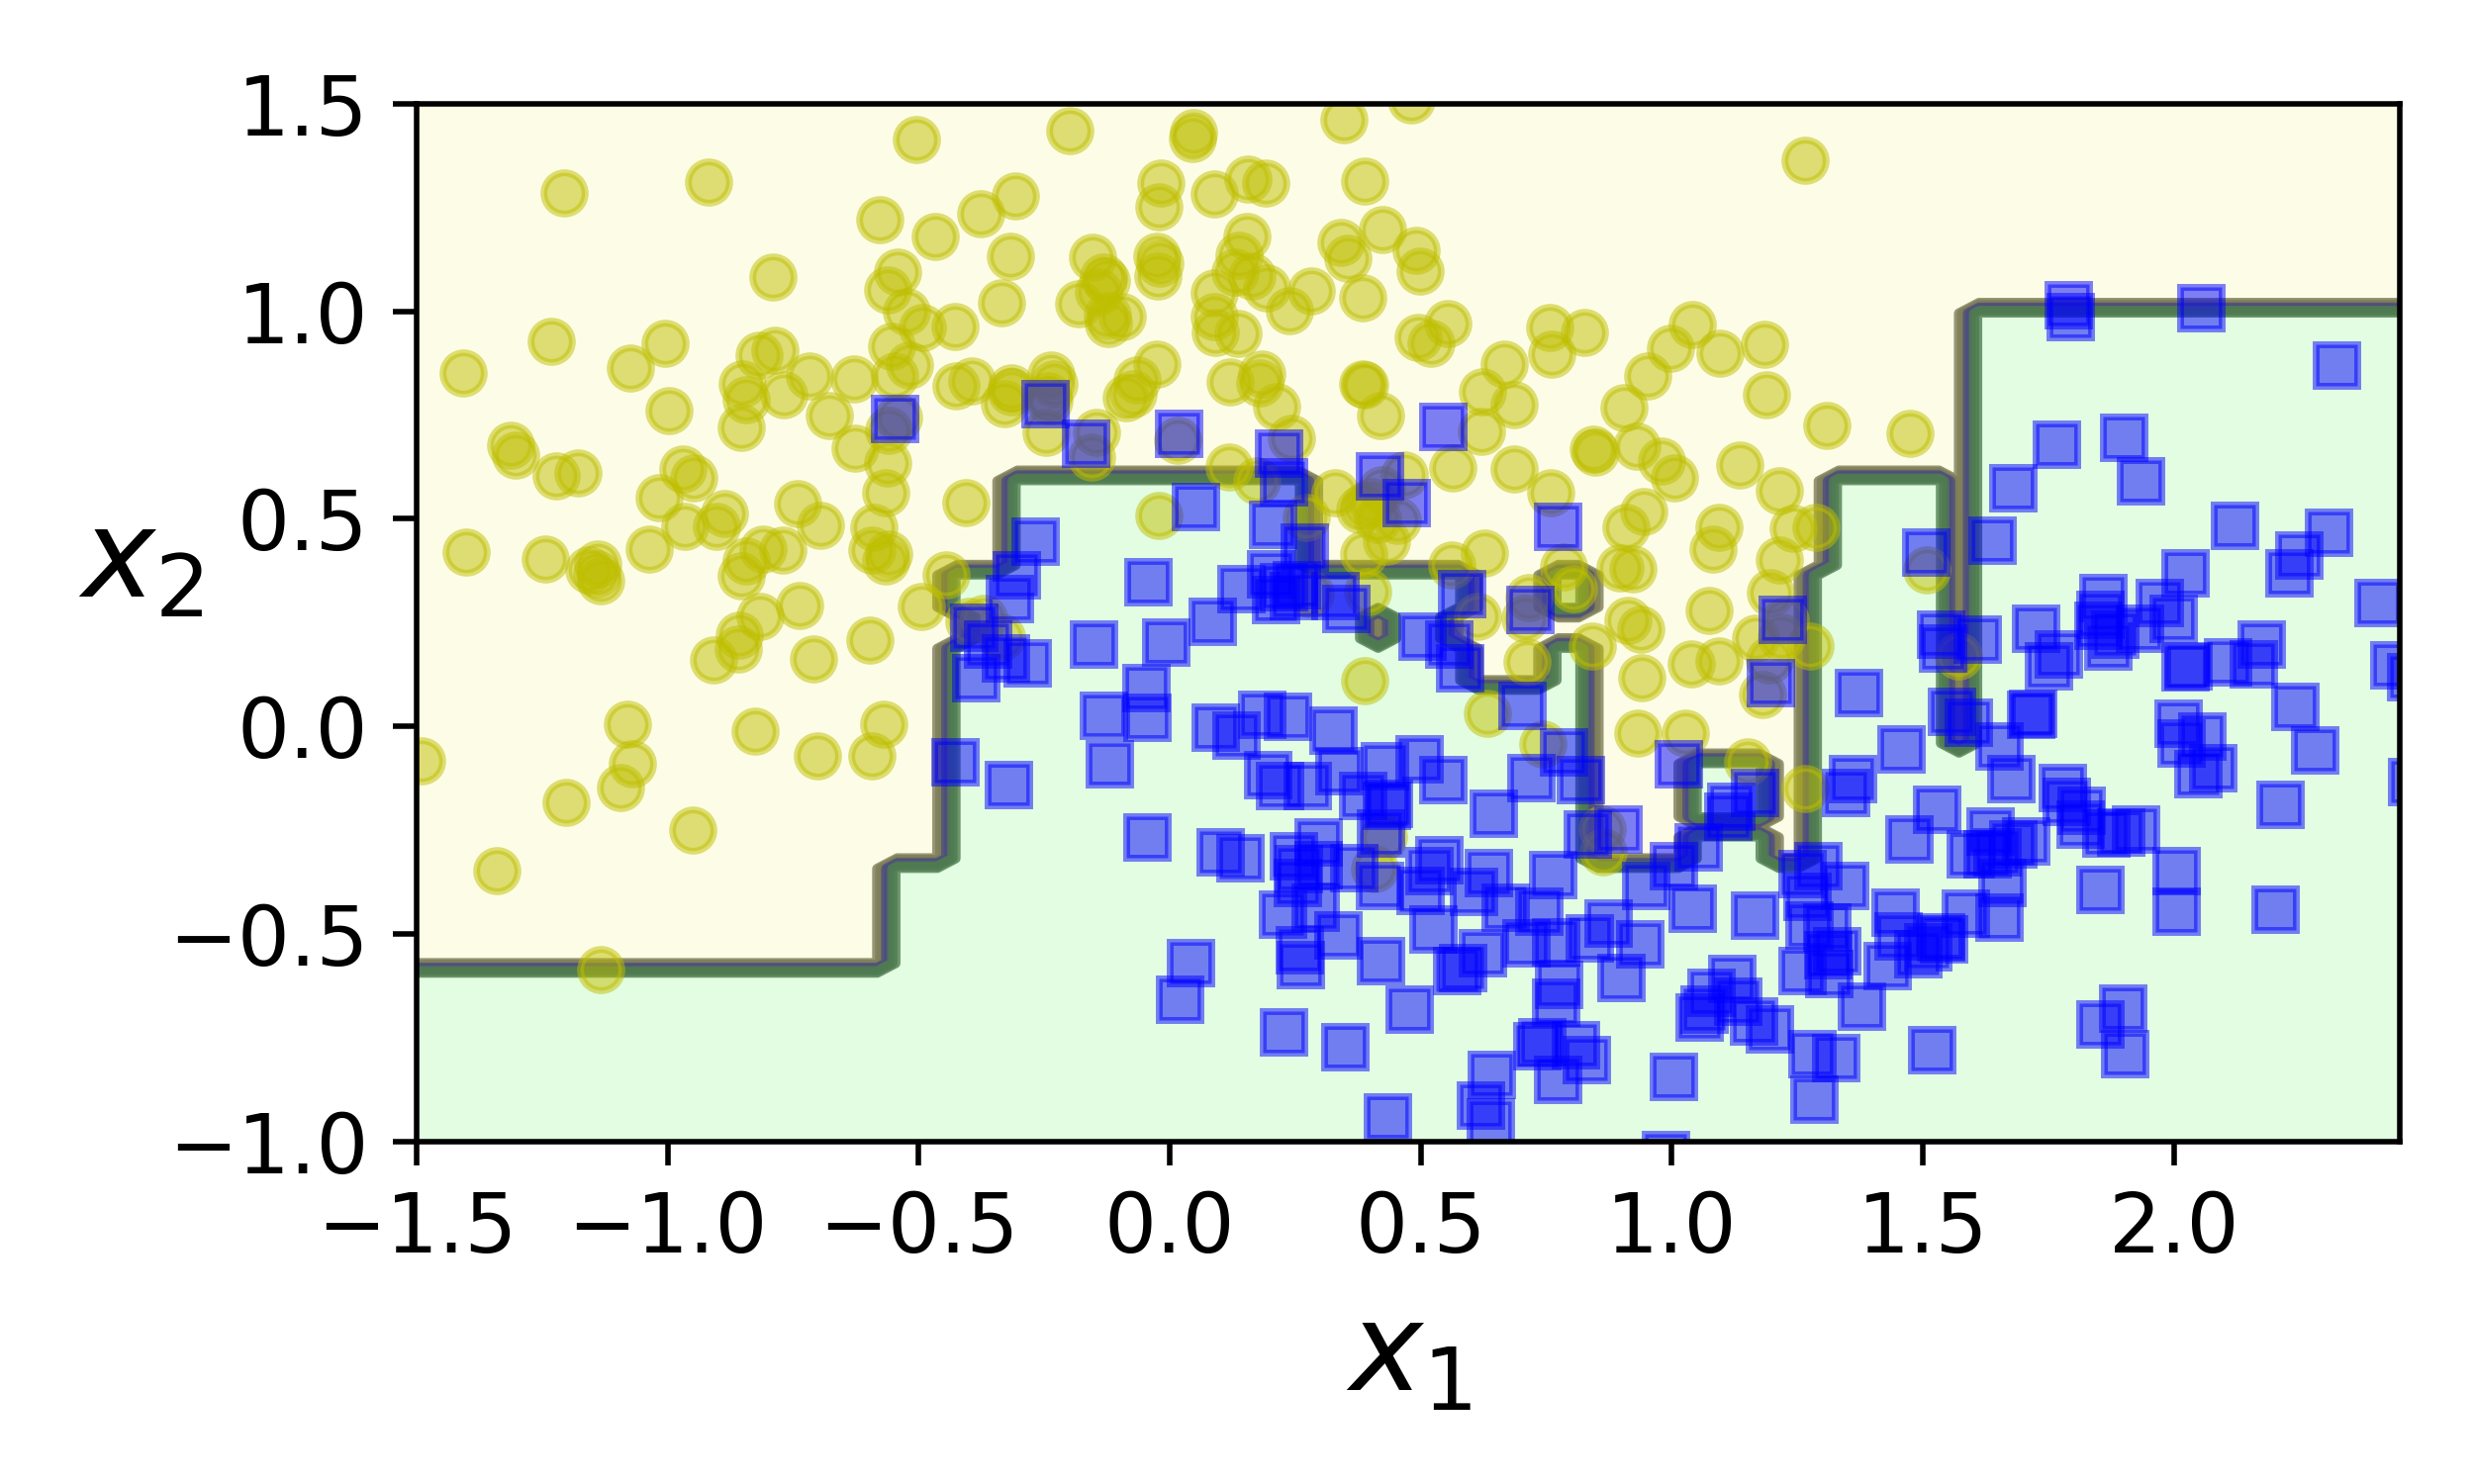
\includegraphics[width=7cm, height=7cm, keepaspectratio]{images/ensemble_8.png}
\end{center}
\end{column}
\end{columns}
\end{frame}

\section{Gradiens turbózás}

\begin{frame}
\tableofcontents[currentsection]
\end{frame}

\begin{frame}{Gradiens turbózás (GBDT)}
Együttes tanuló algoritmus, amely a rezidumok szekvenciális javításával állítja elő a becsült értéket. Minden újonnan létrejövő modell javít az elődje hibáján.\par\medskip
\only<1>{A becsült érték előállítása:\par
\begin{block}{}
\begin{center}
\texttt{Becsült érték = előző predikció + tanulási sebesség * rezidum}
\end{center}
\end{block}
\begin{center}
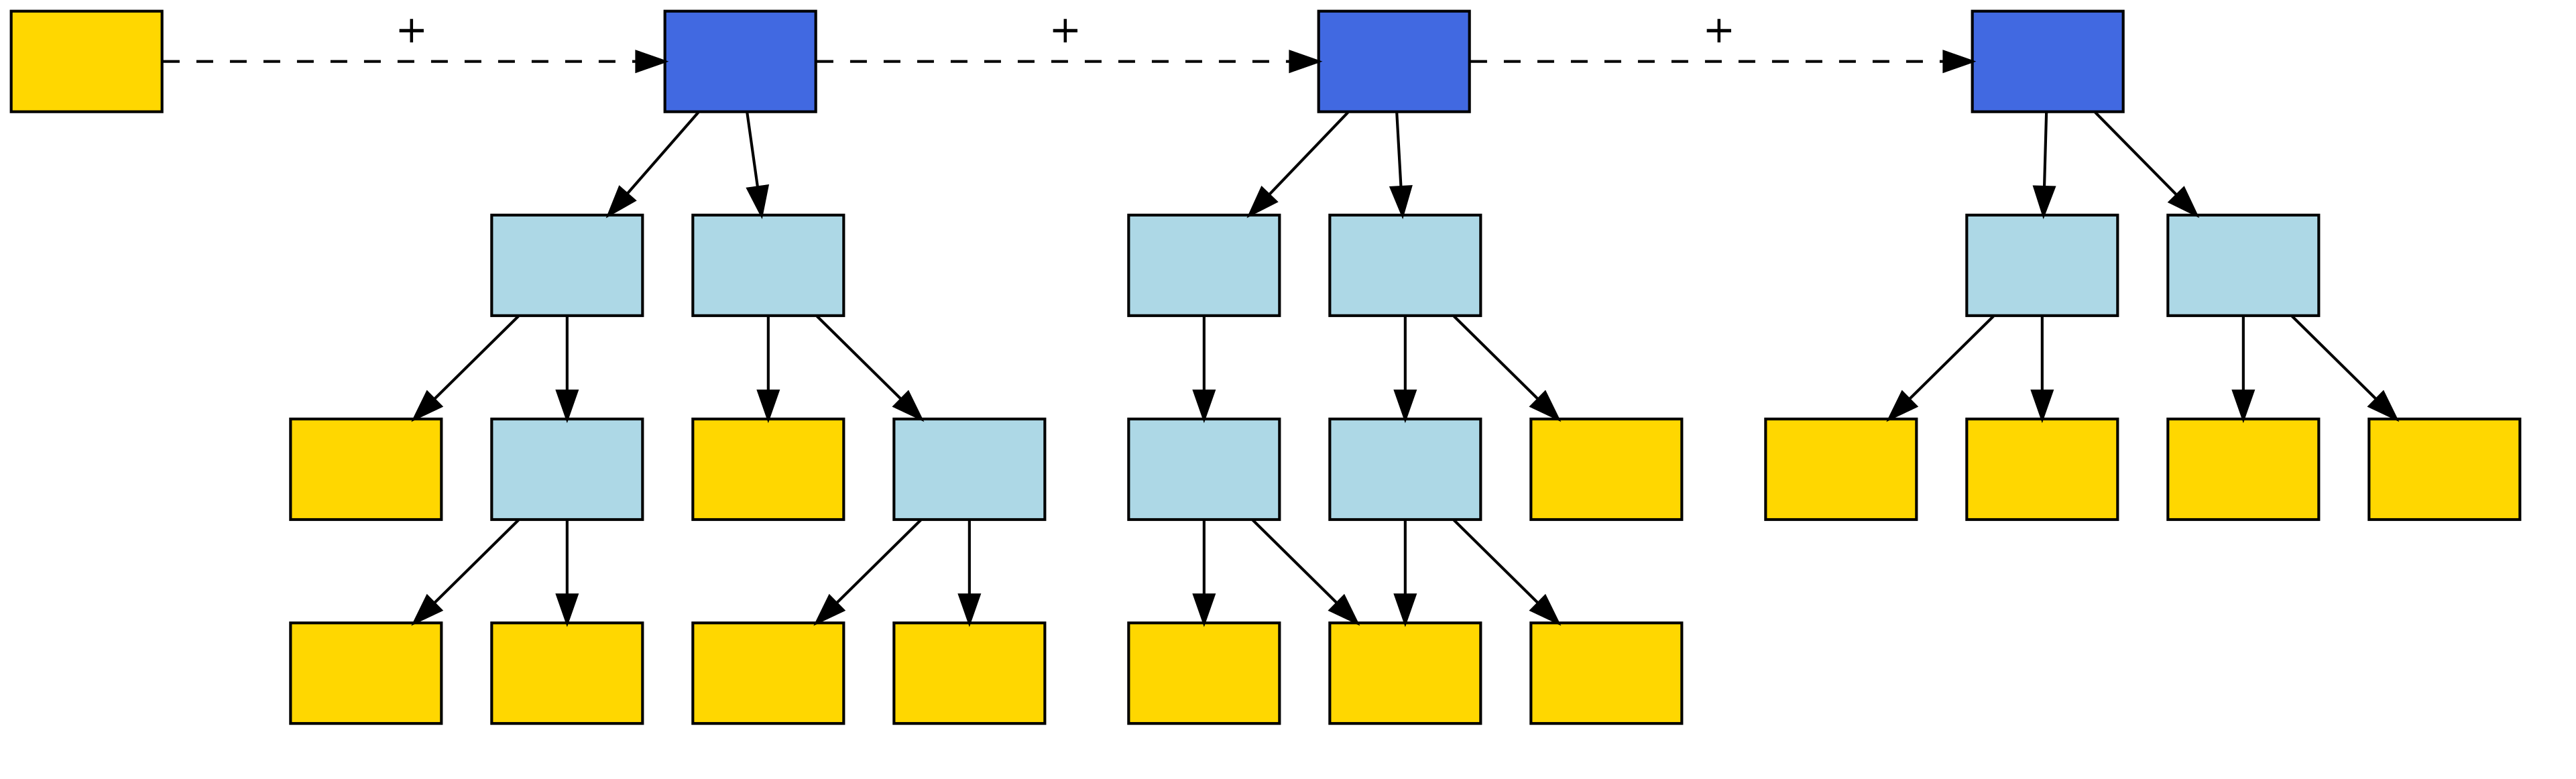
\includegraphics[width=14cm, height=7cm, keepaspectratio]{graphs/ensemble_4.png}
\end{center}}
\only<2>{\begin{algorithm}[H]
\caption{Gradiens turbózás}
\SetAlgoLined
\begin{enumerate}
	\item Kezdeti predikció a célváltozóra
	\item Rezidumok kiszámítása
	\item Döntési fa illesztése a rezidumokra
	\item Levelek output értékének kiszámítása
	\item Predikció a minta adathalmazra
	\item 2-5 lépés iterálása kilépésig
\end{enumerate}
\end{algorithm}}
\end{frame}

\begin{frame}{Gradiens turbózás: lépésről lépésre}
\begin{columns}
\begin{column}{.5\textwidth}
\begin{enumerate}
	\item A GBDT egy adott $y$ célváltozóra vonatkozó első predikciója a célváltozó várható értéke:
\end{enumerate}
\begin{block}{}
\[
F_0\left(x\right) = \underset{\gamma}{argmin} \sum_{i=1}^n L\left(y_i, \gamma\right)
\]
Ahol:
\begin{itemize}
	\item $L\left(y, \gamma \right)$: Deriválható költségfüggvény
	\item $\gamma$: Az az érték, ami minimalizálja a mintaegyedekre kiszámolt rezidumok összegét
\end{itemize}
\end{block}
\end{column}
\begin{column}{.5\textwidth}
\begin{center}
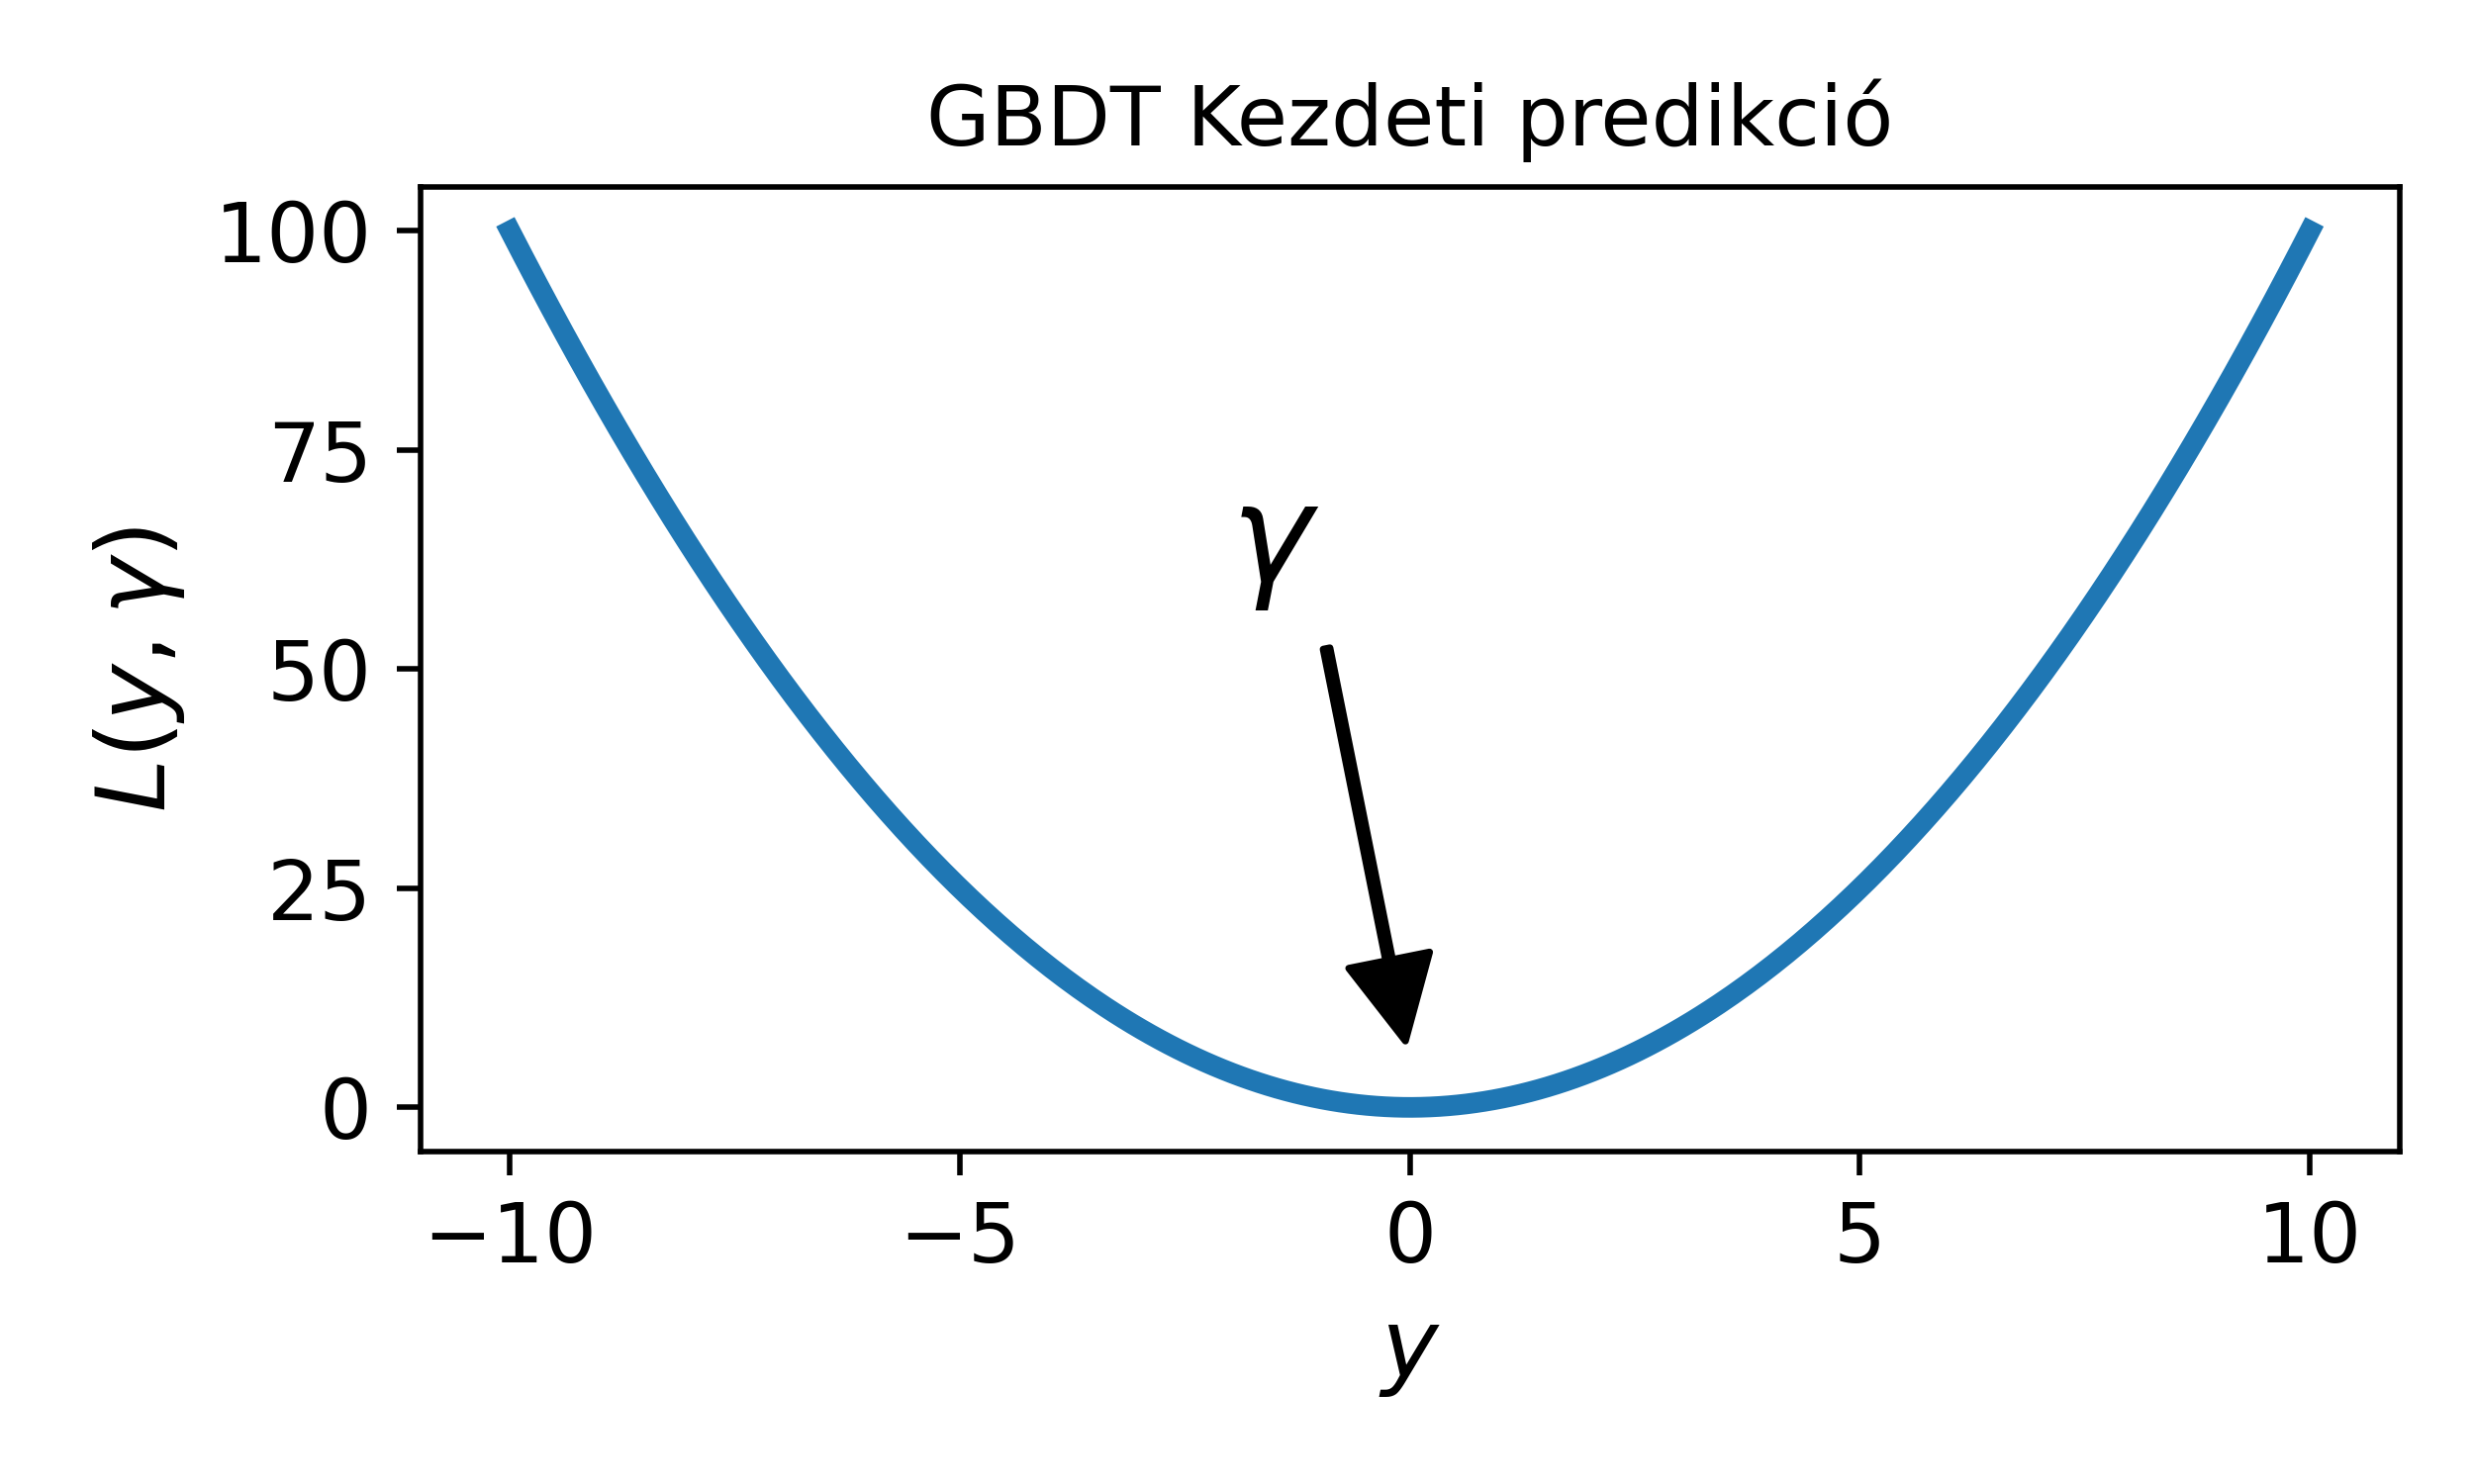
\includegraphics[width=7cm, height=7cm, keepaspectratio]{images/ensemble_10.png}
\end{center}
\end{column}
\end{columns}
\end{frame}

\begin{frame}{Gradiens turbózás: lépésről lépésre}
\begin{columns}
\begin{column}{.45\textwidth}
\begin{enumerate}
	\setcounter{enumi}{1}
	\item Következőnek az algoritmus kiszámolja a rezidumokat minden mintaegyedre. A rezidum a becsült és valós érték különbsége adott $L$ költségfüggvény szerint:
\end{enumerate}
	\begin{block}{Rezidum}
	\[
	r_{i,m} = -\left[ \frac{\partial L\left(y_i, F\left(x_i\right)\right)}{\partial F \left( x_i \right)} \right]_{F\left( x \right) = F_{m-1}\left( x \right)}
	\]
	Ahol:
	\begin{itemize}
		\item $i$: A minta indexe
		\item $m$: A modell indexe
	\end{itemize}
	\end{block}
\end{column}
\begin{column}{.55\textwidth}
\begin{center}
\begin{small}
\begin{tabular}{|c|c|c|c|c|}
\hline
Magasság & Szemszín & Nem & Súly & Rezidum \\ \hline
$1.6$      & Kék      & Férfi & $88$  & $16.8$   \\ \hline
$1.6$      & Barna    & Nő    & $76$  & $4.8$    \\ \hline
$1.5$      & Kék      & Nő    & $56$  & $-15.2$  \\ \hline
$1.8$      & Zöld     & Férfi & $73$  & $1.8$    \\ \hline
$1.5$      & Barna    & Férfi & $77$  & $5.8$    \\ \hline
$1.4$      & Kék      & Nő    & $57$  & $-14.2$  \\ \hline
\end{tabular}
\end{small}
\[
F_0(x) = \frac{1}{6} \left( 88+76+56+73+77+57 \right) = 71.2
\]
\[
r_{1,1} = 88 - 71.2 = 16.8
\]
\[
r_{1,2} = 76 - 71.2 = 4.8
\]
\end{center}
\end{column}
\end{columns}
\end{frame}

\begin{frame}{Gradiens turbózás: lépésről lépésre}
\begin{columns}
\begin{column}{.5\textwidth}
\begin{enumerate}
	\setcounter{enumi}{2}
	\item Döntési fa illesztése a \textbf{rezidumokra}. Ebben a lépésben az algoritmus besorolja a rezidumokat egy döntési fa leveleibe. 
\end{enumerate}
\begin{center}
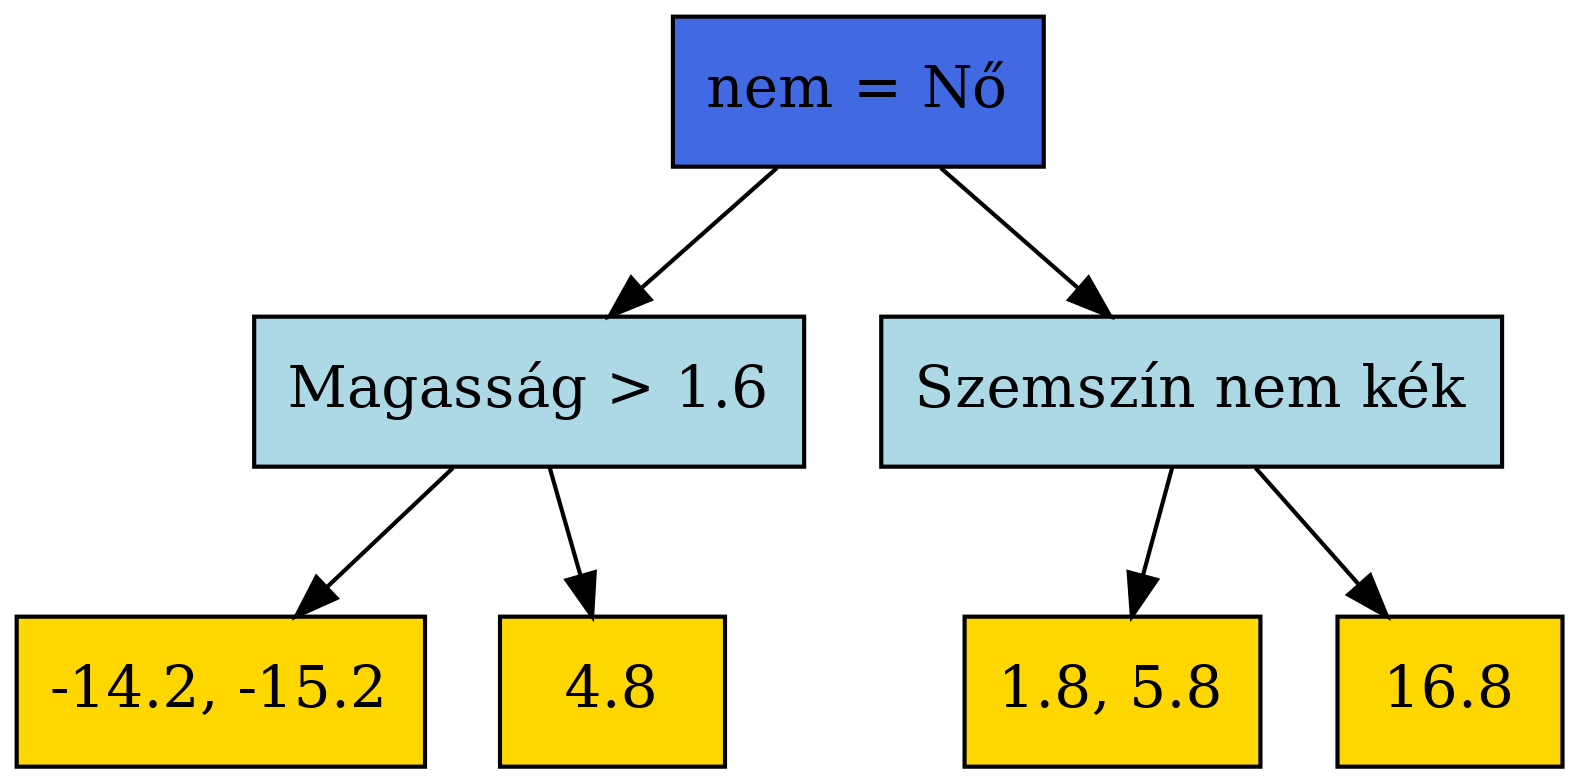
\includegraphics[width=7cm, height=7cm, keepaspectratio]{graphs/ensemble_5.png}
\end{center}
\end{column}
\begin{column}{.5\textwidth}
\begin{center}
\begin{small}
\begin{tabular}{|c|c|c|c|c|}
\hline
Magasság & Szemszín & Nem & Súly & Rezidum \\ \hline
$1.6$      & Kék      & Férfi & $88$  & $16.8$   \\ \hline
$1.6$      & Barna    & Nő    & $76$  & $4.8$    \\ \hline
$1.5$      & Kék      & Nő    & $56$  & $-15.2$  \\ \hline
$1.8$      & Zöld     & Férfi & $73$  & $1.8$    \\ \hline
$1.5$      & Barna    & Férfi & $77$  & $5.8$    \\ \hline
$1.4$      & Kék      & Nő    & $57$  & $-14.2$  \\ \hline
\end{tabular}
\end{small}
\end{center}
\end{column}
\end{columns}
\end{frame}

\begin{frame}{Gradiens turbózás: lépésről lépésre}
\begin{columns}
\begin{column}{.5\textwidth}
\begin{enumerate}
	\setcounter{enumi}{3}
	\item Levelek output értékének kiszámítása: a levelek outputja az az érték, ami minimalizálja a levélbe bekerült értékekre a költségfüggvényt. Ez az esetek többségében a rezidumok átlaga. 
\end{enumerate}
\begin{center}
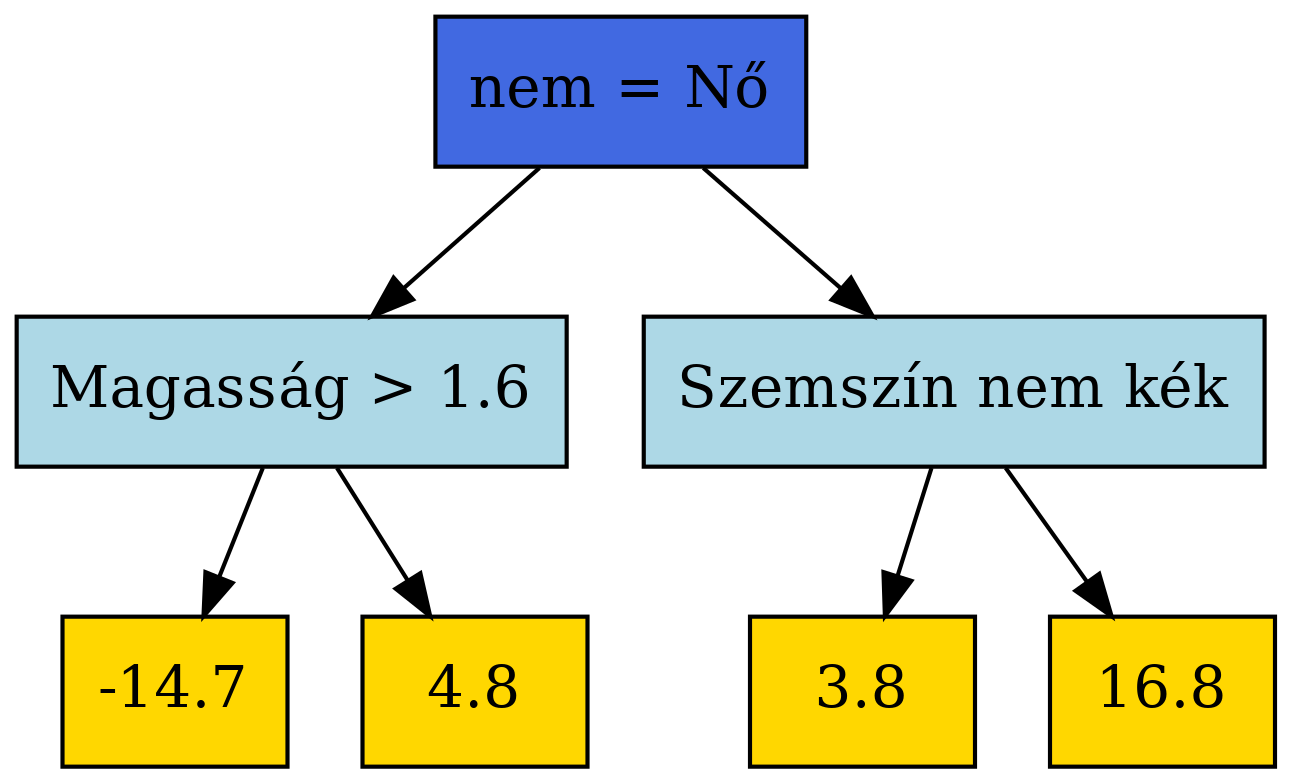
\includegraphics[width=6cm, height=7cm, keepaspectratio]{graphs/ensemble_6.png}
\end{center}
\end{column}
\begin{column}{.5\textwidth}
\begin{block}{Levél output}
\[
\gamma_{j,m} = \underset{\gamma}{argmin} \sum_{x_i \in R_{i,j}} L\left( y_i, F_{m-1}\left( x_i \right) + \gamma \right)
\]
Ahol:
\begin{itemize}
	\item $\gamma$: A levél outputja
	\item $F_{m-1}x_i$: A modell előző fája által adott predikció $x_i$ egyedre. 
	\item $y_i$: A célváltozó valós értéke
\end{itemize}
\end{block}
\end{column}
\end{columns}
\end{frame}

\begin{frame}{Gradiens turbózás: lépésről lépésre}
\begin{columns}
\begin{column}{.5\textwidth}
\begin{enumerate}
	\setcounter{enumi}{4}
	\item Predikciók készítése a minta adathalmazra
\end{enumerate}
\begin{block}{GBDT Predikció}
\[
F_m\left( x \right) = F_{m-1}\left( x \right) + \alpha \sum_{j=1}^{J_m} \gamma_{j,m}\;\; x \in R_{j,m}
\]
Ahol:
\begin{itemize}
	\item $F_{m-1}\left( x \right)$: Az $x$ mintaegyedre az előző fa által adott becsült érték
	\item $\alpha$: A tanulási sebesség
	\item $J$: A levelek száma
\end{itemize}
\end{block}
\end{column}
\begin{column}{.5\textwidth}
A predikció az első mintaegyedre $\alpha = 0.1$ tanulási sebességgel:
\vspace{-0.5cm}
\begin{center}
\begin{small}
\begin{tabular}{|c|c|c|c|c|}
\hline
Magasság & Szemszín & Nem & Súly & Rezidum \\ \hline
$1.6$      & Kék      & Férfi & $88$  & $16.8$   \\ \hline
\end{tabular}
\end{small}
\end{center}
\begin{center}
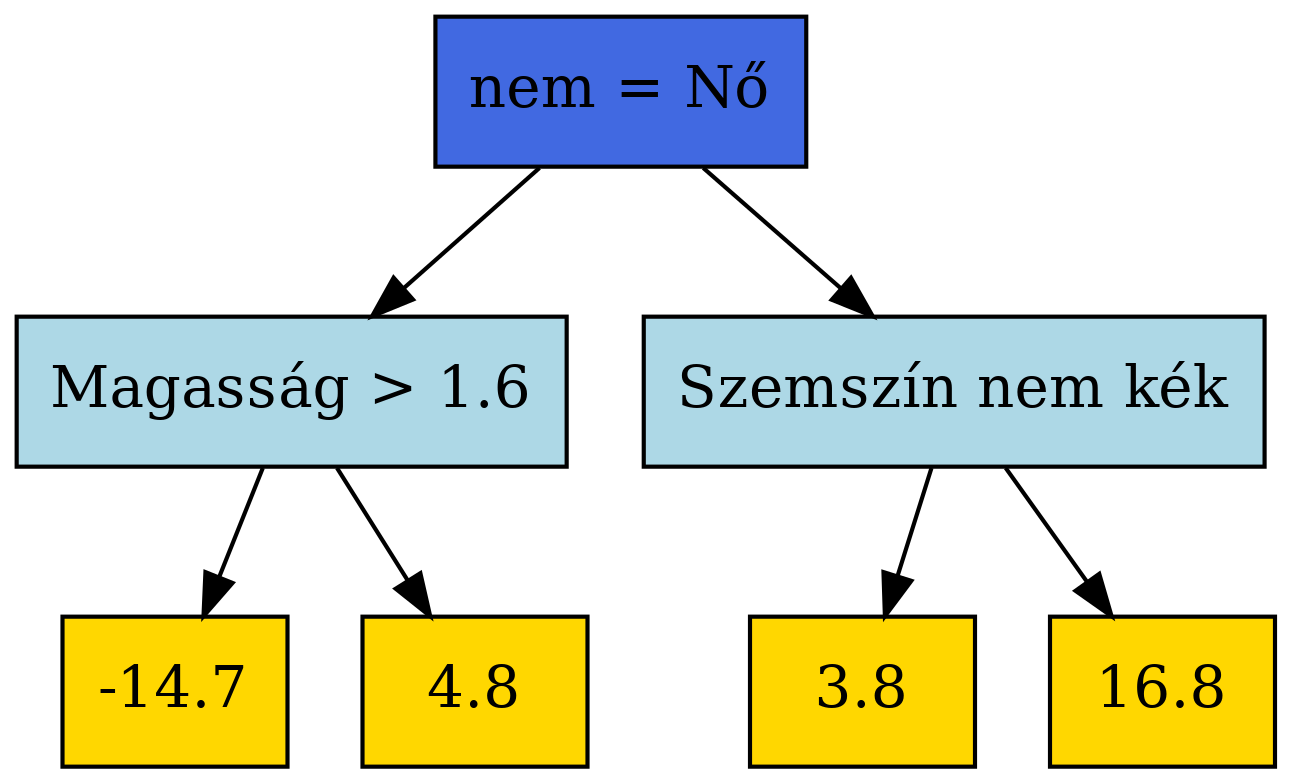
\includegraphics[width=5cm, height=7cm, keepaspectratio]{graphs/ensemble_6.png}
\end{center}
$F_0\left( x \right) = 71.2$
$F_1\left( x \right) = 71.2 + 0.1 \cdot 16.8 = 72.9$
\end{column}
\end{columns}
\end{frame}

\begin{frame}{Gradiens turbózás: lépésről lépésre}
Az $F_1\left( x \right)$ predikciója alapján a következő rezidumok minden mintaegyedre:
\begin{center}
\begin{small}
\begin{tabular}{|c|c|c|c|c|c|}
\hline
Magasság & Szemszín & Nem & Súly & Rezidum $r_{i,1}$ & Rezidum $r_{i,2}$\\ \hline
$1.6$      & Kék      & Férfi & $88$  & $16.8$  & $15.1$  \\ \hline
$1.6$      & Barna    & Nő    & $76$  & $4.8$   & $4.3$   \\ \hline
$1.5$      & Kék      & Nő    & $56$  & $-15.2$ & $-13.7$ \\ \hline
$1.8$      & Zöld     & Férfi & $73$  & $1.8$   & $1.4$   \\ \hline
$1.5$      & Barna    & Férfi & $77$  & $5.8$   & $5.4$   \\ \hline
$1.4$      & Kék      & Nő    & $57$  & $-14.2$ & $-12.7$ \\ \hline
\end{tabular}
\end{small}
\[
r_{1,2} = 88 - \left(71.2 + 0.1 \cdot 16.8 \right) = 15.1
\]
\[
r_{2,2} = 76 - \left(71.2 + 0.1 \cdot 4.8 \right) = 4.3
\]
\end{center}
\end{frame}

\begin{frame}{Gradiens turbózás: lépésről lépésre}
Miután létrejöttek az $r_{i,2}$ rezidumok ismételten besorolódnak egy döntési fába.\par\medskip
\begin{columns}
\begin{column}{.5\textwidth}
Az első döntési fa:
\begin{center}
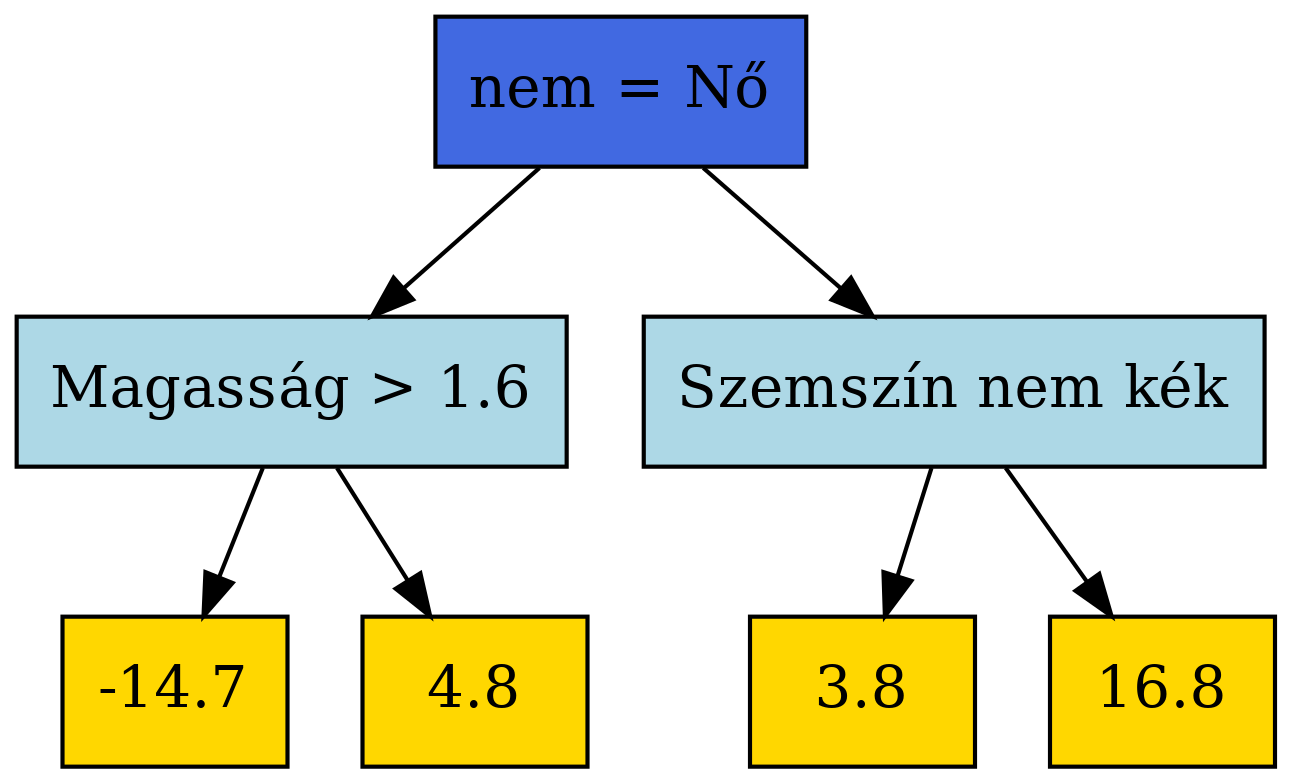
\includegraphics[width=7cm, height=7cm, keepaspectratio]{graphs/ensemble_6.png}
\end{center}
\end{column}
\begin{column}{.5\textwidth}
A második döntési fa:
\begin{center}
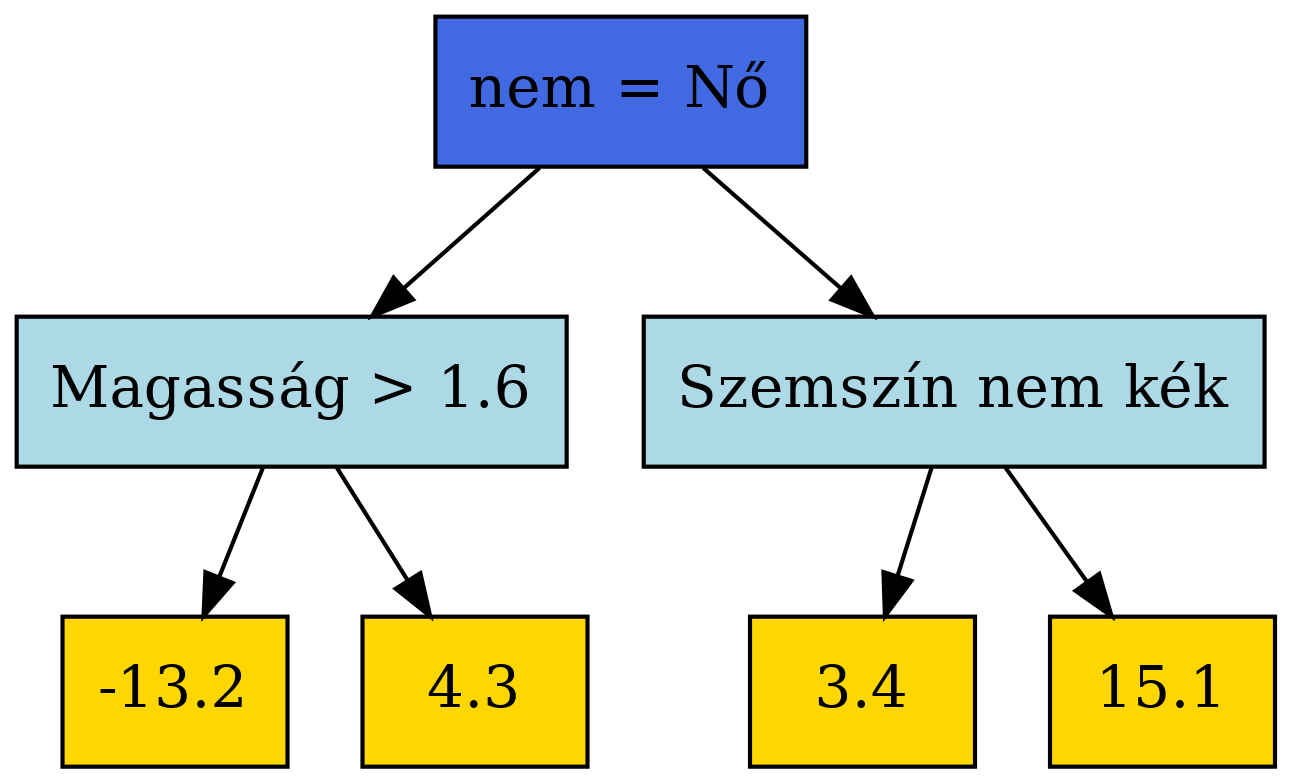
\includegraphics[width=7cm, height=7cm, keepaspectratio]{graphs/ensemble_7.png}
\end{center}
\end{column}
\end{columns}
\end{frame}

\begin{frame}{Tanítás lépései egy minta adathalmazon}
\begin{center}
\includegraphics<1>[width=14cm, keepaspectratio]{images/ensemble_11.png}
\includegraphics<2>[width=14cm, keepaspectratio]{images/ensemble_12.png}
\includegraphics<3>[width=14cm, keepaspectratio]{images/ensemble_13.png}
\end{center}
\end{frame}

\begin{frame}{Alultanulás és túltanulás}
\begin{columns}
\begin{column}{.4\textwidth}
A turbózott regresszor fák is hajlamosak a túltanulásra.\par\medskip
A tanító feladata felismerni a túltanulás jelenségét és vagy \textbf{az egyéni fák korlátozásával, vagy a tanítási időszakok rövidítésével regularizálni a modellcsoportot}.\par\medskip
A bal oldali ábrán egy alultanult, a jobb oldalin pedig egy túltanult modell predikciói láthatók.
\end{column}
\begin{column}{.6\textwidth}
\begin{center}
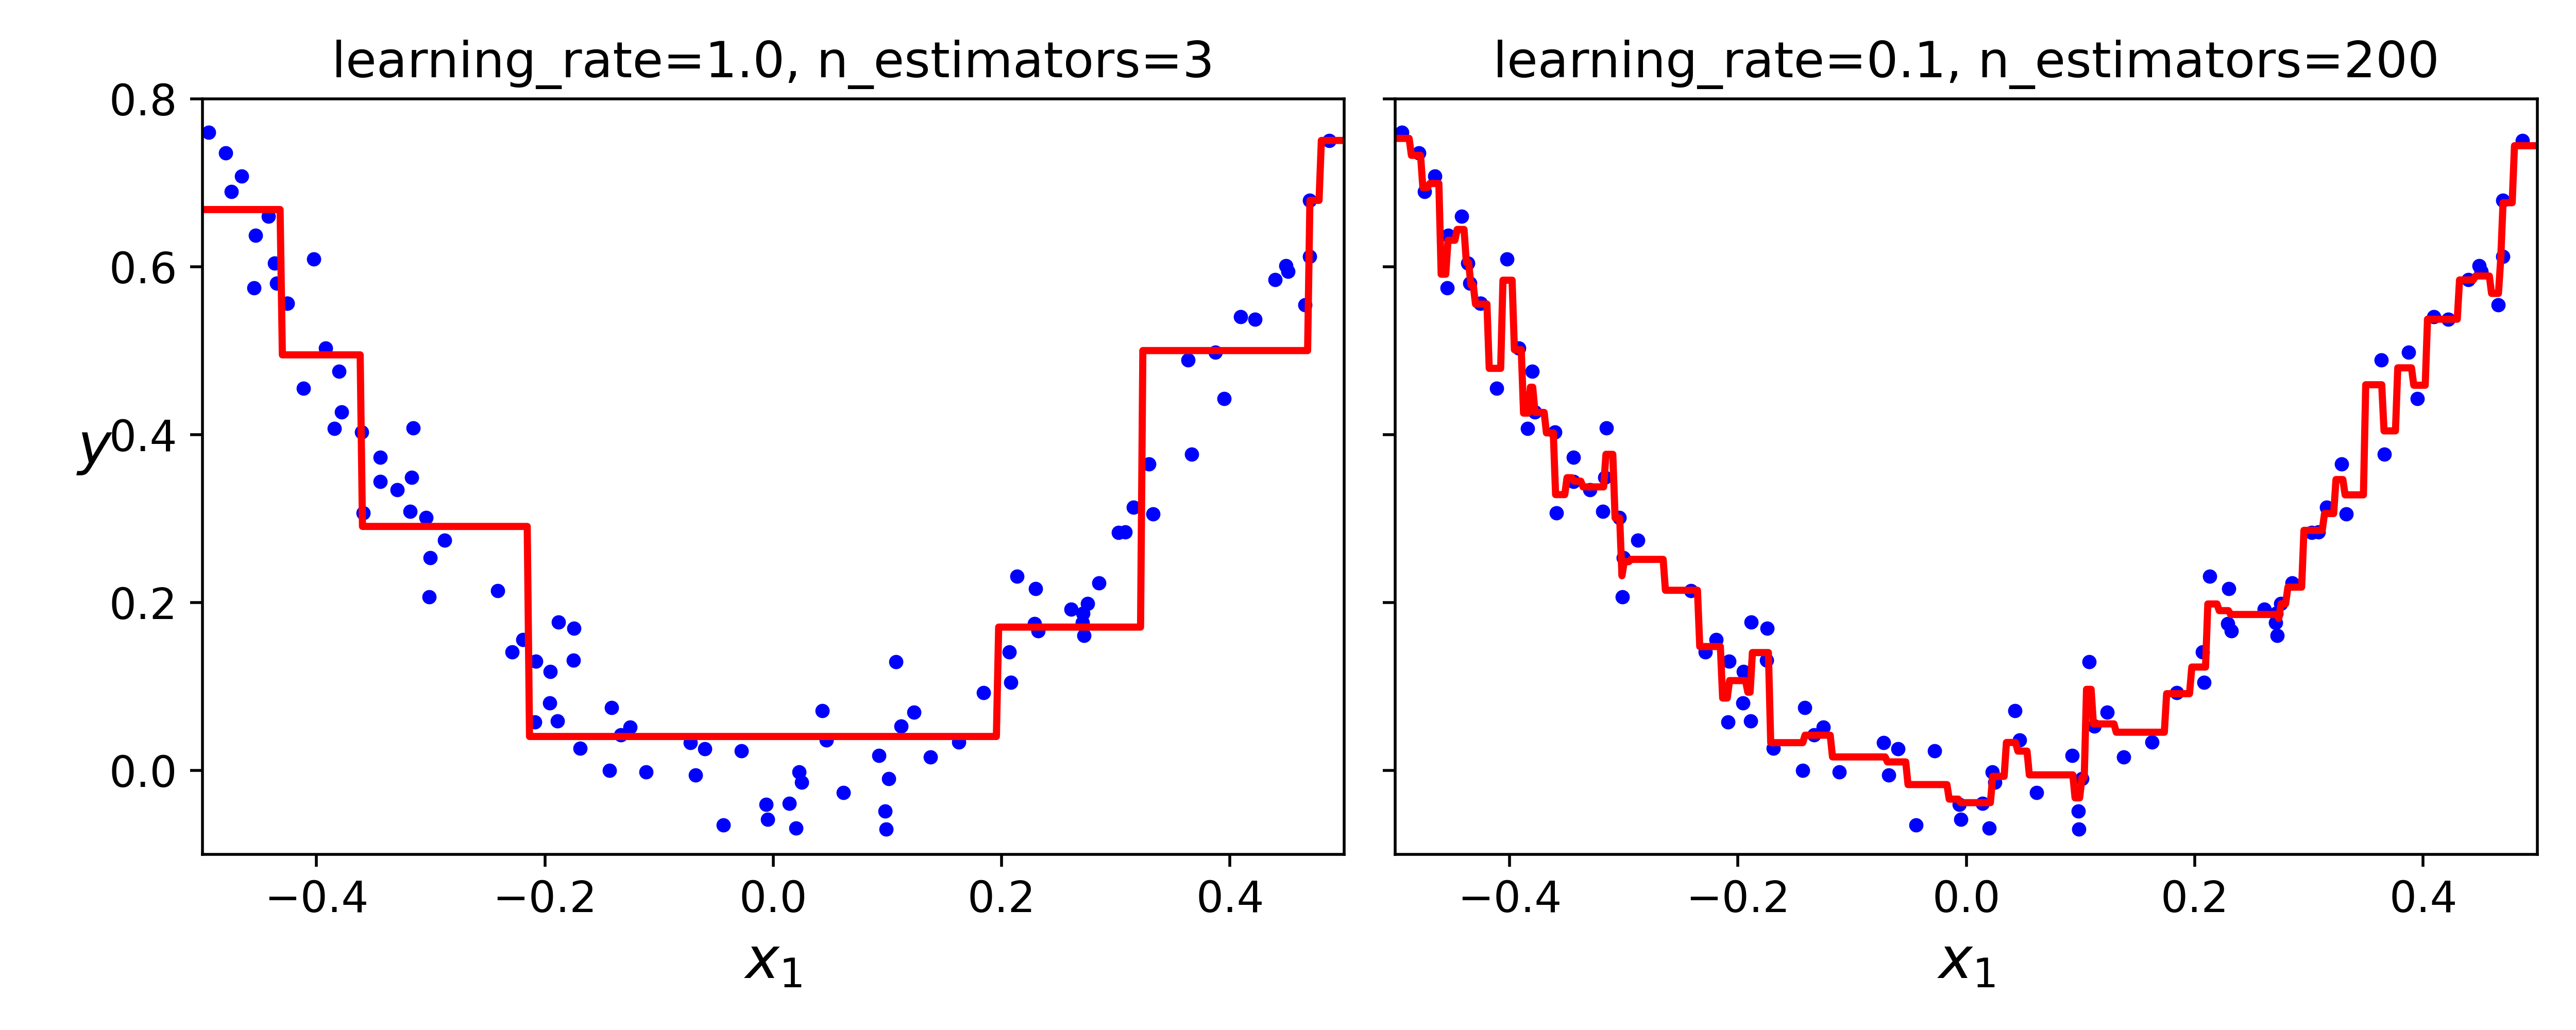
\includegraphics[width=9cm, height=7cm, keepaspectratio]{images/ensemble_14.png}
\end{center}
\end{column}
\end{columns}
\end{frame}

\begin{frame}{Korai leállás gradiens turbózással}
Korai leállás implementálása segíthet elkerülni a túltanulást. Ilyenkor az a modell lesz a végleges, amelyik a legkisebb validációs hibát érte el. Ha a validációs hiba emelkedőn van, a tanító iteráció kilép. 
\begin{center}
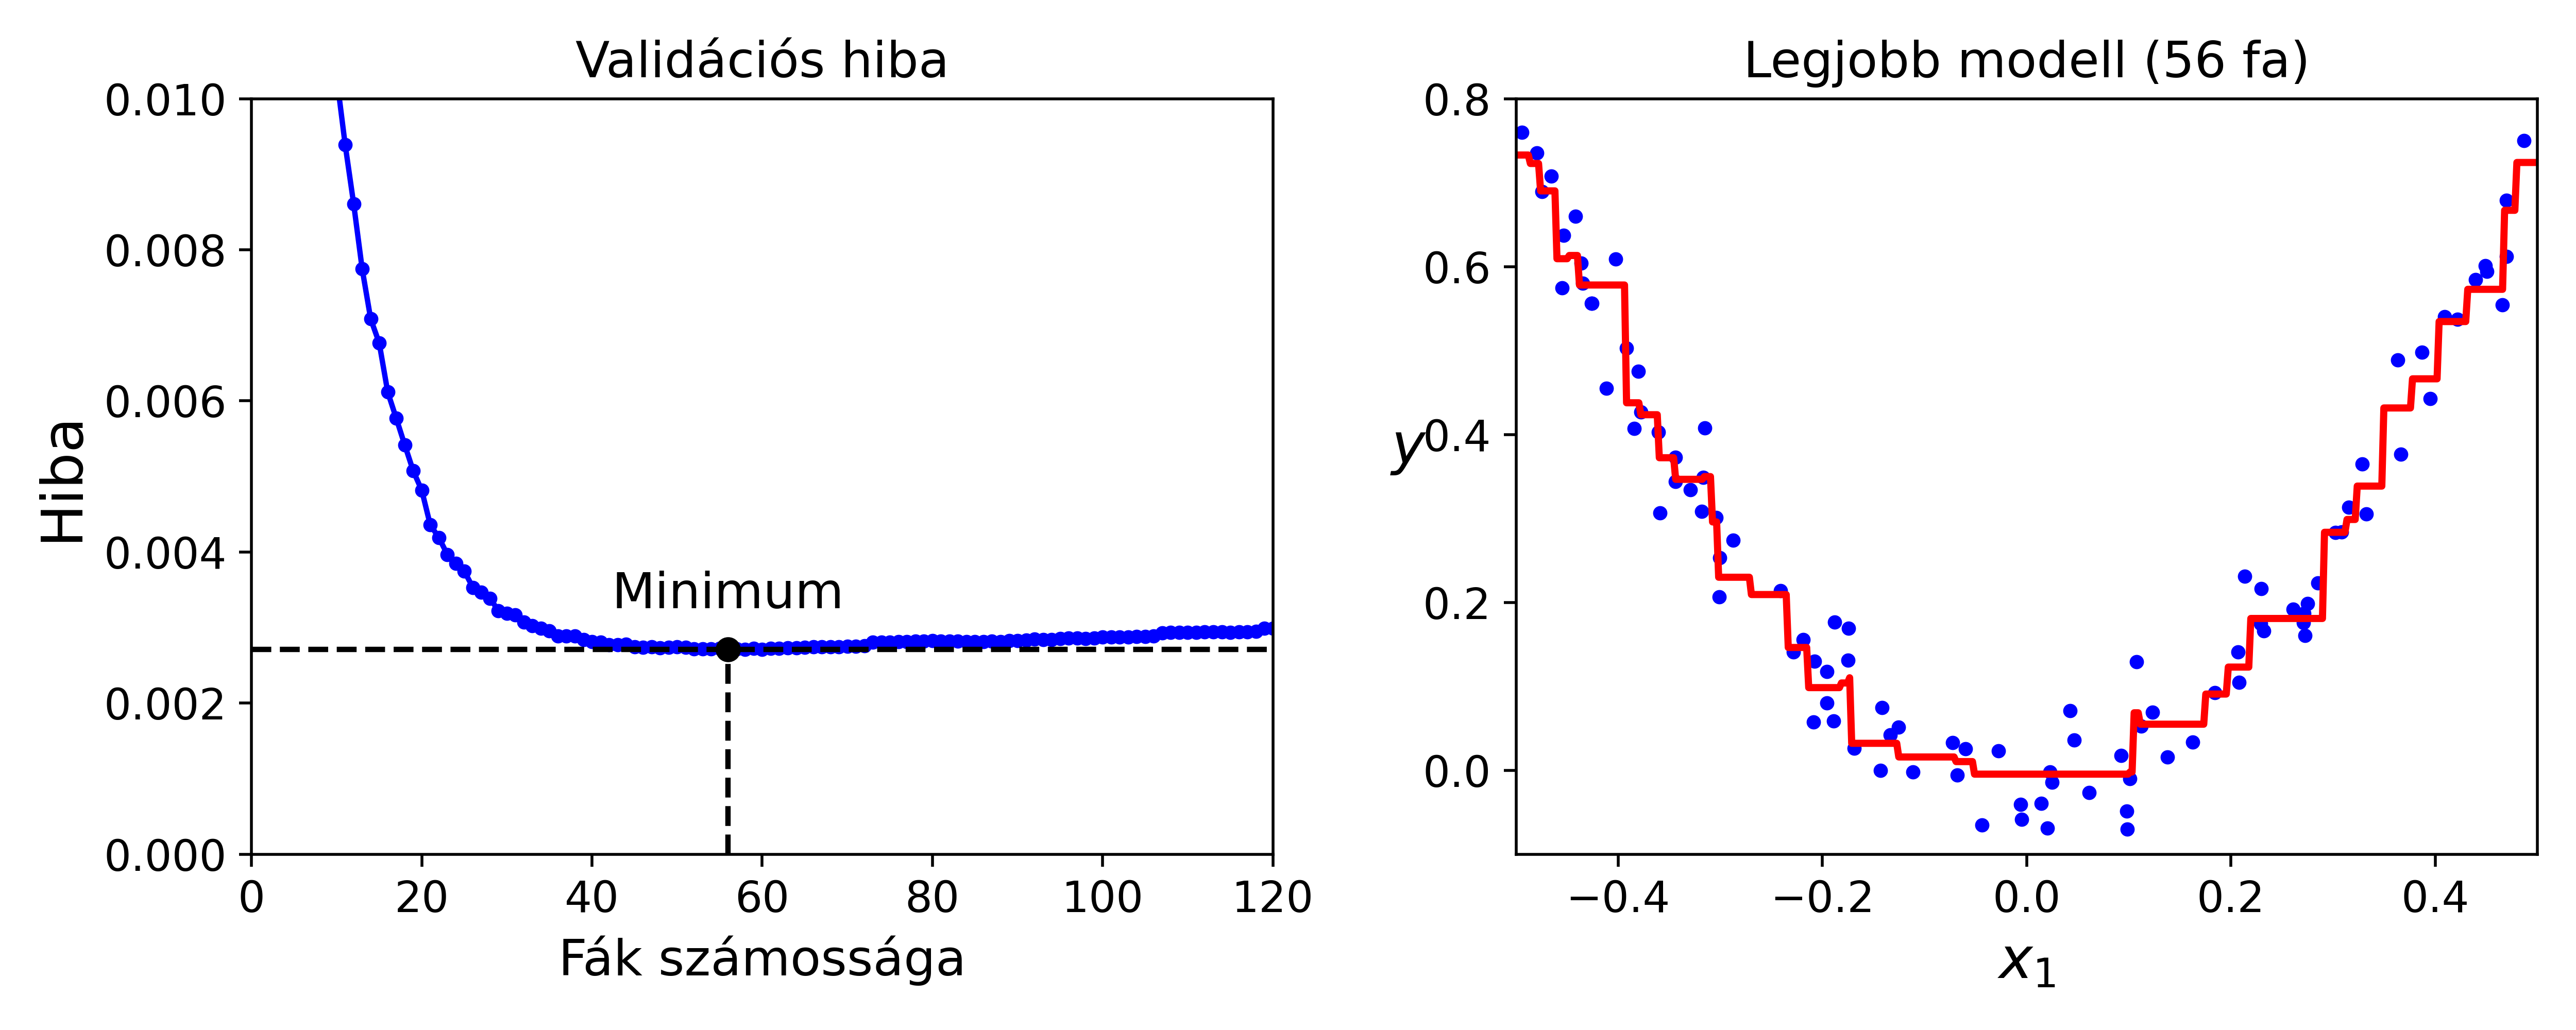
\includegraphics[width=13cm, keepaspectratio]{images/ensemble_15.png}
\end{center}
\end{frame}

\end{document}


























